%**********************************************************************
% Base layout + including standard packages
%**********************************************************************
\documentclass[a4paper,12pt]{report}

\usepackage[utf8]{inputenc}	% allows direct input of special chars
\usepackage{setspace}		% permits to set space between lines

% ensure proper appearance of all fonts in pdf:
\usepackage[T1]{fontenc}
%\usepackage{lmodern}		% lmodern after T1 fontenc (_may_ be required)
%\usepackage{times} -- obsolete; use:
\usepackage{mathptmx}		% Times as default text font, maths support
\usepackage{courier}		% provides bold font (required for syntax highlighting in listings)

\usepackage{multirow}		% enables table cells to span multiple rows

\usepackage{parskip}		% paragraphs: no indentation at beginning, but spacing between

\usepackage[pdftex]{graphicx}
\DeclareGraphicsExtensions{.pdf,.jpg,.png}


%**********************************************************************
% Including non-standard packages
%**********************************************************************

\usepackage{acronym}

\usepackage[usenames,dvipsnames,table]{xcolor}	% http://en.wikibooks.org/wiki/LaTeX/Colors
\definecolor{gray20}{gray}{0.8}
\definecolor{gray5}{gray}{0.95}
\definecolor{olivegreen30}{RGB}{155,187,89}	% from table template in MS Word

\usepackage{alltt}

\usepackage{listings}
\lstset{
	numbers=left, 					% numbers=none if required
	basicstyle=\footnotesize\ttfamily,	
	showstringspaces=false,
	captionpos=b, 					% captionpos=b: caption at bottom
	breaklines=false, 
	numbersep=5pt,
	breaklines=true,
	showspaces=false,
	breaklines=true,
	columns=fixed,
	keepspaces=true,}					

% Geometry as defined by FH guidelines:
\usepackage[top=3cm, bottom=3cm, left=3.5cm, right=3cm]{geometry}

\usepackage{paralist} 		% inline lists
%\usepackage{mdwlist}
\usepackage{enumitem}

\usepackage{float}
\floatstyle{plain}
\restylefloat{figure}
%\usepackage{subfig}
\usepackage{subfigure}
\usepackage{textcomp}		% symbols such as \texttimes and \texteuro
%\usepackage{amssymb}		% math. symbols from the American Mathematical Society

\usepackage[Lenny]{fncychap}	% chapter heading styles
% usepackage[english]{babel}	% adjust to your needs (if not specified: US English)

% Biblatex
% ---------------------------------------------------------------------
\usepackage{csquotes}		% context sensitive quotation; recommended for usage with Biblatex
%% Note: date, origdate, eventdate, and urldate require yyyy-mm-dd format
%% dd or mm-dd may be omitted
\usepackage[
    backend=biber,
    urldate=long,		% default: short, e.g. 08/15/2010
    style=authoryear,	% Harvard citation style
%   sorting=nty		this is default: sort by name, title, year
%   sortlocale=de_DE	set according to your needs
    natbib=true,		% if you want to use natbib compatible citation commands; do _not_ use package natbib!
    maxbibnames=1000,		% show all authors in the bibliography
]{biblatex}
% Strict Harvard style: URL date default is "(Visited on ...)"; so:
% These two BibTeX entries
%	url = {http://...},
%	urldate = {2015-03} -- or 2015, or 2015-03-31
% shall be printed as
%	Available from: <http://...> [March 2015]
\DeclareFieldFormat{urldate}{\mkbibbrackets{#1}}
\DeclareFieldFormat{url}{Available\space from\addcolon\space <\url{#1}>}
\addbibresource{references.bib}
% ---------------------------------------------------------------------
\usepackage[			% hyperref should be last package loaded
    pdftex,			% driver
    pdftitle={<Title of Your Thesis>},
    pdfsubject={Master's Thesis},
    pdfauthor={<your name>},
    breaklinks,			% permits line breaks for long links
    bookmarks,			% create Adobe bookmarks
    bookmarksnumbered,		% ... and include section numbers
    linktocpage,		% "make page number, not text, be link on TOC ..."
    colorlinks,			% yes ...
    linkcolor=black,		% normal internal links;
    anchorcolor=black,		% don't make scientific papers too much colourful => "black"
    citecolor=black,
    urlcolor=blue,		% quite common
    pdfstartview={Fit},		% "Fit" fits the page to the window
    pdfpagemode=UseOutlines,	% open bookmarks in Acrobat
    plainpages=false,		% avoids duplicate page number problem
    pdfpagelabels,
  ]{hyperref}

%**********************************************************************
% Layout adjustments
%**********************************************************************

% page layout (header/footer and page numbers)
%\pagestyle{empty}
\pagestyle{headings}
%\pagestyle{fancy}

% settings for structure
\setcounter{secnumdepth}{3}
%\setcounter{tocdepth}{2}
\setcounter{tocdepth}{1}

%**********************************************************************
% LaTeX macros and commands
%**********************************************************************

% new command to start a chapter (no page number)
\newcommand{\chapterstart}{\thispagestyle{empty}}

% new command to close a chapter (flush, i.e. print remaining figures and tables)
\newcommand{\chapterend}{\newpage{\pagestyle{empty}\cleardoublepage}}

% new environment for smaller paragraphs
\newenvironment{spar}
{\begingroup \leftskip 0.7cm \rightskip\leftskip}
{\par \endgroup}
% ^^^ must be set here (or use empty line)



%**********************************************************************
% Special hyphenation rules
%**********************************************************************

\hyphenation{JOANNEUM}		% extend to your needs

%**********************************************************************
% Structure of thesis: inclusion of chapters
%**********************************************************************

\begin{document}

% define languages *******************************************************

\lstdefinelanguage{swift}
{
  morekeywords={
    func,if,then,else,for,in,while,do,switch,case,default,where,break,continue,fallthrough,return,
    typealias,struct,class,enum,protocol,var,func,let,get,set,willSet,didSet,inout,init,deinit,extension,
    subscript,prefix,operator,infix,postfix,precedence,associativity,left,right,none,convenience,dynamic,
    final,lazy,mutating,nonmutating,optional,override,required,static,unowned,safe,weak,internal,
    private,public,is,as,self,unsafe,dynamicType,true,false,nil,Type,Protocol, import},
  morecomment=[l]{//}, % l is for line comment
  morecomment=[s]{/*}{*/}, % s is for start and end delimiter
  morestring=[b]" % defines that strings are enclosed in double quotes
}

\definecolor{keyword}{HTML}{BA2CA3}
\definecolor{string}{HTML}{D12F1B}
\definecolor{comment}{HTML}{008400}
\definecolor{darkgreen}{HTML}{008400}
\definecolor{lightgray}{rgb}{.9,.9,.9}
\definecolor{darkgray}{rgb}{.4,.4,.4}
\definecolor{purple}{rgb}{0.65, 0.12, 0.82}

\lstdefinelanguage{JavaScript}{
  keywords={typeof, new, true, false, catch, function, return, null, catch, switch, var, if, in, while, do, else, case, break, const},
  ndkeywords={class, export, boolean, throw, implements, import, this, bodyPartial, exports},
  sensitive=false,
  comment=[l]{//},
  morecomment=[s]{/*}{*/},
  morestring=[b]',
  morestring=[b]"
}

%end languages***********************************************************

%Command to lstset Swift Code
\newcommand{\swiftcode}{
	\lstset{
		language=swift,
		basicstyle=\footnotesize\ttfamily,
		keywordstyle=\color{keyword}\bfseries,
		stringstyle=\color{darkgreen},
		commentstyle=\color{darkgray},
	}
}
% end language command**************************************************

  %**********************************************************************
% right side, if two-sided
\chapterend

\begin{titlepage}

\begin{center}
% scale image according to the actual logo you use
% official JPG ist way too large, so [height=2.5cm] is required
% official EPS, converted to PDF:

\includegraphics[height=1cm]{images/logo_FHJ_100mm_cmyk}
\hfill

% the actual title
\mbox{}\vfill

  \large

  {\huge\bf Swift on Linux}

  \vspace{2.0cm}

  {\bf Project Work}\\
submitted in conformity with the requirements for the grade of\\
{\bf lecture "Projektarbeit"}\\
in the Bachelor degree programme {\bf Software Design\\}

  \vspace{0.5cm}

 FH JOANNEUM  (University of Applied Sciences), Kapfenberg

  \vspace{1.5cm}

  \mbox{}

  {\bf Supervisor: DI Johannes Feiner, FH JOANNEUM Kapfenberg

  submitted by: Stefan Moder, Christian Hofer\\
  personnel identifier: 1510418049, 1510418043}

  \vspace{1.5cm}

   July 2017

\end{center}
\vfill\mbox{}


\end{titlepage}


%**********************************************************************

% right side/flush
\chapterend

\begin{titlepage}

\begin{center}\large\bf
Assignment for the project work of\\
Stefan Moder, Christian Hofer\\
Matr. no. 1510418049, 1510418043
\\[2ex]
Subject:\\
``Swift on Linux''
\end{center}

\begin{abstract}
Write your abstract here.

Kapfenberg, 24.07.2017\\[1.5ex]
{\bf Academic adviser:}\\
DI Johannes Feiner

\flushright
% Here your name serves as signature
\vspace{15mm}
Stefan Moder, Christian Hofer
\end{abstract}

\end{titlepage}


%**********************************************************************

% right side
\chapterend

\begin{titlepage}

%-t-\parindent0pt
%-t-\parskip1.5ex plus.5ex minus.5ex

\begin{center}\large\bf
Formal declaration
\end{center}

We hereby declare that we have produced the present work by ourself and without any aids other than those mentioned herein. Any ideas taken directly or indirectly from third party sources are indicated as such. This paper has not been published or submitted to any other examination board in the same or a similar form.

\vspace{1,5cm}
Kapfenberg, 24.07.2017

\flushright
\vspace{15mm}
Stefan Moder, Christian Hofer

\end{titlepage}


%**********************************************************************

\chapterend

\begin{titlepage}

\begin{center}\large\bf
Acknowledgement
\end{center}
Thanks to \ldots

\end{titlepage}


%**********************************************************************

\chapterend


  \pagenumbering{roman}		% roman page numbers for title pages

  \tableofcontents
  \listoftables
  \listoffigures
  \chapterend

  \pagenumbering{arabic}	% ... for ordinary chapters
  \onehalfspacing
  %%%%%%%%%%%%%%%%%%%%%%%%%%%%%%%%%%%%%%%%%%%%%%%%%%%%%%%%%%%%%%%%%%%%%%%%%%%%%
\chapter{Introduction}\label{chap:introduction}
%%%%%%%%%%%%%%%%%%%%%%%%%%%%%%%%%%%%%%%%%%%%%%%%%%%%%%%%%%%%%%%%%%%%%%%%%%%%%
\chapterstart
\section{Kurzfassung}
\label{section:kurzfassung}
\paragraph{Kurzfassung}
In dieser Arbeit wurde mit Hilfe des Perfect Frameworks ein Webserver auf einem Ubuntu Server 16.04 LTS erstellt. Zur Implementierung wurde die open-source Programmiersprache Swift in der Version 3.1.1 verwendet. Der implementierte Server wurde mit einem Webserver auf Basis des Express.js Frameworks verglichen. Zur Dokumentation des Projektes wurde ein WikiBook erstellt, welches beschreibt, wie man allgemein einen Webserver mit Swift auf Linux erstellt.
\paragraph{Abstract}
In this work a webserver on the basis of the Perfect Framework was implemented. As programming language, open source Swift at version 3.1.1 was used for the implementation. The Webserver runs on a Ubuntu Server 16.04 LTS. Further, the implementation was compared to anthor implementation of the same server based on the Express.js Framework. As the documentation of the project a wikibook was produced, which details the step to creating a web server with swift on a Linux mashin. 
% Einleitung
\section{Einleitung}
\label{sec:einleitung}
Das Ziel dieser Arbeit ist es einen Webserver mit Hilfe der Programmiersprache Swift auf einem Linux-Server zu entwickeln. 
\subsection{Swift}
\label{subsection:swift}
Swift ist die noch junge Programmiersprache von Apple, welche als Nachfolger von Objective-C gedacht ist. Die Sprache ist objektorientiert, stark typisiert, mit Typinfernce, mutliparadigmen-orientierte, kompilierende, all zwecks Programmiersprache. Die Frameworks Cocoa und Cocoa Touch funktionieren mit Swift und Bruecken zu Objective-C sind in die Sprache integriert. Der Swift-Code selbst soll dabei praezise und doch gleichzeitig ausdrucksstark sein\parencite{appleswift}.  Die Programmiersprache wurde auf der WWDC (Apple's World Wide Developer Conference)\parencite{swiftannounced} enthuellt. Swift wurde ueber Jahre hinweg produziert und wird immer noch weiterentwickelt. Zur Zeit ist Swift auf Version 4\parencite{ swift4}. Im \textit{TIOBE Index}\parencite{tiobe} liegt Swift auf Platz 12 hinter Go (Platz 10) und Perl (Platz 11), aber vor Ruby (Platz 13). Auch ist dem Index zu entnehmen, dass sich Swift um zwei Plaetze verbessert hat. In der \textit{Developer Survey} von stackoverflow schafft es Swift auf Platz 11 der meist benutzen Programmiersprachen und im Ranking der Beliebtesten sogar auf Platz 4 vor Go und Python\parencite{survey2017}. Im Jahr zuvor war Swift bei der Beliebtheit sogar auf Platz 2\parencite{survey2016}. Besonders die Verwendbarkeit von Swift fuer alle Arten von Projekten, von iOS Development, ueber systemnahe Programmierung, mobile Apps, bis hin zu Cloud Technologien, sorgen fuer eine hohe Beliebtheit. Genauso wie die Sicherheit von Swift, wie durch automatische Speicherverwaltung, Array Indexes werden auf out-of-bound Zugriffe geprueft, Optionals erzwingen die Behandlung von moeglichen nil-Werten und Variablen sind immer initialisiert. Andererseits scheinen bestimmte Teile der Programmiersprache wie Closures, Error-Handling und Optional gerade Einsteigern das Erlernen von Swift zu erschweren\parencite{studyonswift}.
\paragraph{Basics of Swift}
\label{para:basicsofswift}
Um die Sprache zu verstehen, beziehungsweisse um die Erlernbarkeit zu beurteilen folgt nun eine kleine Einfuehrung basierend auf \textit{The Swift Programming Language}\parencite{swiftbook}.
Swift kennt Konstanten und Variablen, wobei durch eine Doppelpunkt getrennt der Typ annotiert wird. Wenn moeglich kann der Typ auch inferiert werden.
\lstset{
	caption=Variablen und Konstanten,
	label=lst:variablenundkonstanten,
	language=swift,
	basicstyle=\footnotesize\ttfamily,
	keywordstyle=\color{keyword}\bfseries,
	stringstyle=\color{darkgreen},
	commentstyle=\color{darkgray},
}
\begin{lstlisting}
	var : String = "Swift"  // Ein String
	var = "FH-Joanneum"  // Auch ein String durch Typinferenz
 	let = "Linux"  // Eine Konstante
	var x = 0, y = 1, z = 3  // Mehrere Variablen in einer Zeile
\end{lstlisting}
Als naechstes Kollektionen. Swift kennt Array, Set, Dictionary. Diese sind standardmaessig "mutable", das heisst aenderbar, wird aber die Kollektion als \lstinline{let} sprich Konstante initialisiert, wird sie unveraenderbar.
\lstset{
	caption=Array\, Set\, Dictionary,
	label=lst:arraysetdictionary,
	language=swift,
	basicstyle=\footnotesize\ttfamily,
	keywordstyle=\color{keyword}\bfseries,
	stringstyle=\color{darkgreen},
	commentstyle=\color{darkgray},
}
\begin{lstlisting}
var intarray = [Int]()   // Ein Array aus Integern
var stringarray = ["Bier", "Wein", "Wasser"] // Array bereits mit Werten gefuellt
let anotherone = [Int]()	// Immutable Array
var intset = Set<Int>()	// Ein Set, der Typ muss hashbar sein
var dictionary = [Int: String]()  // Ein Dictionary mit einem Key (Int) Value(String) Paar
\end{lstlisting}
Der Kontrollfluss wird in Swift aehnlich zu anderen Sprachen geregelt. Swift kennt \lstinline{for}, \lstinline{while}, \lstinline{if} und \lstinline{switch}.

\lstset{
	caption=Kontrollfluss,
	label=lst:kontrollfluss,
	language=swift,
	basicstyle=\footnotesize\ttfamily,
	keywordstyle=\color{keyword}\bfseries,
	stringstyle=\color{darkgreen},
	commentstyle=\color{darkgray},
}
\begin{lstlisting}
let demo = ["Eins", "Zwei", "Drei", "Vier"]
// Ein for-Loop
for number in demo {
	print("Nummer = \(number)!") // print() schreibt in die Konsole
} 
// Ausgabe
// Nummer = Eins!
// Nummer = Zwei!
// Nummer = Drei!
// Nummer = Vier!
var  counter = 0
var max = 2
// Ein while-Loop
while counter < max {
	print( "Der Zaehler ist \(counter)")
	counter = counter + 1
} 
// Ausgabe
// Der Zaehler ist 0
// Der Zaehler ist 1\\
// repeat while
repeat {
	print( "Der Zaehler ist \(counter)")
} while counter > 0 
// Ausgabe
// Der Zaehler ist 1
// Der Zaehler ist 0\\
var age = 19
// If Abfragen
if age >= 18 { // Eine Altersabfrage
   print("Hier ist ein Bier") 
   // ueber 18 bekommt man Bier
} else {
  print ("Hier ist ein Glass mit Wasser") 
  // Unter 18 ein Glass Wasser
}\\
let char: Character = "F"
// Switch Case
switch char {
    case "A":
	// Hier ist der Code fuer A
    case "B", "C":
	// Hier ist der Code fuer B und C
    case "F":
	print("Der Code von F")
	fallthrough 
	// Der nachfolgende Case wird auch ausgefuehrt
    case "D":
	print("Der Code von D")
    default:
	// Wenn nichts passt
} 
// Ausgabe
// Der Code von F
// Der Code von D\\
// Label und break
outer: while true { // while-Loop mit Label
	for i in 0..<100 { // Wuerde von 0 bis 99 zaehlen
		print("Index \(i)")
		break outer 
		// Bricht beide Loops und springt zum Label
	}
} 
// Ausgabe
// Index 0
\end{lstlisting} 
Funktionen in Swift bestehen aus Funktionsname, Parameter (eventuell mit Label) und Rueckgabewert. Funktionen haben nur einen Rueckgabewert, dieser kann aber ein Optional sein, bzw. koennen Funktionen auch Fehler werfen.
\lstset{
	caption=Funktionen,
	label=lst:funktionen,
	language=swift,
	basicstyle=\footnotesize\ttfamily,
	keywordstyle=\color{keyword}\bfseries,
	stringstyle=\color{darkgreen},
	commentstyle=\color{darkgray},
}
\begin{lstlisting}
// Eine Funktion die einen String als Parameter bekommt
// und einen String zurueck gibt
// "sag" ist das Label des Parameters
// "name" ist der Name der Variable
func einefunktion(sag name: String) -> String {
	print("Name = \(name)")
	return "Ein String als Rueckgabewert"
}
// Aufruf
einefunktion(sag: "Bert")
// Ausgabe (der Rueckgabewert wird hier ignoriert)
// Name = Bert
\\
\\
// Mit _ kann das Label beim Aufruf unterdrueckt werden
// Void als Rueckgabewert bedeutet kein Rueckgabewert
func keinlabel( _ name: String) -> Void {
	print("Name = \(name)")
}
// Aufruf
keinlabel("Hugo") 	// Name = Hugo
einefunktion(sag: "Hugo") // Name = Hugo

// In-Out Parameters erlaubt Parameter in der
// Funktion zu aendern, sofern 
//diese keine Konstanten sind
func wechseldich(wechsel name: inout String) {
	name = "Bob"
}
// Aufruf
var name = "Billy"
print(name) // Billy
wechseldich(wechsel: name)
print(name) // Bob
\end{lstlisting}

Der naechste Punkt ist Closures, diese entsprechen in etwa Lambda-Ausdruecken. Diese erlauben Callback-Funktionen direkt inline zu definieren.
\lstset{
	caption=Closures,
	label=lst:closures,
	language=swift,
	basicstyle=\footnotesize\ttfamily,
	keywordstyle=\color{keyword}\bfseries,
	stringstyle=\color{darkgreen},
	commentstyle=\color{darkgray},
}
\begin{lstlisting}
// Diese Funktion benoetigt eine Callback Funktion
func function(callback: (String)->Void) {
	callback("Gruss von der Funktion")
}
// Und hier der Aufruf mittels Closure
function(callback: { s in print(s) }) // Gruss von der Funktion
// Oder in der Trailing-Variante
function(callback: (String) -> Void ) {
	s in print("Trailing \(s)")
}
\end{lstlisting}
Vor den Klassen und  Strukturen noch eine schnelle Einfuehrung in  Enumerations.
\lstset{
	caption=Enumerations,
	label=lst:enumerations,
	language=swift,
	basicstyle=\footnotesize\ttfamily,
	keywordstyle=\color{keyword}\bfseries,
	stringstyle=\color{darkgreen},
	commentstyle=\color{darkgray},
}
\begin{lstlisting}
// Hier eine Enumeration mit komplexerm Typ
enum FHEntity {
    case student(nr: Int, name: String) 
    case lehrender(name: String)
}
\\
var std = FHEntity.student(nr: 13, name: "Geheim") 
// Lege einen neuen Studenten an
\\
switch std {
    case .student(let nr, let name):
        print("\(name)") // Student
    case .lehrender(let name):
        print("\(name)") // Lehrender
} // Ausgabe Geheim
\end{lstlisting}
Und nun zu Strukturen und Klassen in Swift. Klassen koennen mehr als Strukturen und zwar Vererbung, Type-Casting, Deinitialisierung und ARC. Werden Klassen einer neuen Variable zu geordnet, wird nur die Referenz uebertragen, bei Strukturen wird eine Kopie erstellt.
\lstset{
	caption=Klassen und Strukturen,
	label=lst:klassenundstrukturen,
	language=swift,
	basicstyle=\footnotesize\ttfamily,
	keywordstyle=\color{keyword}\bfseries,
	stringstyle=\color{darkgreen},
	commentstyle=\color{darkgray},
}
\begin{lstlisting}
// Eine einfache Klasse
class A {
    var name: String
    init(_ name: String) {
        self.name = name
    }
}
// Eine Einfache Struktur
struct B {
    var name: String
    init(_ name: String) {
        self.name = name
    }
}
var a = A("Montag") // neue Instanz der Klasse A
var b = B("Jaenner") // neue Struktur B
var newera = a // nur Referenz
var newerb = b // neue Struktur mit kopierten Werten
newera.name = "Dienstag" // neuer Name fuer die Klasse
newerb.name = "Februar" // neuer Name fuer die Struktur
print("Die alte Klasse ist \(a.name) " +
       "die neue ist \(newera.name)")
print("Die alte Struktur ist \(b.name) " +
        "die neue ist \(newerb.name)")
// Die alte Klasse war Dienstag die neue ist Dienstag
// Die alte Struktur war Jaenner die neue ist Februar
\end{lstlisting}
Die Funktionen einer Klasse sind vom Syntax her leicht anders als in anderen Programmiersprachen, aber dafuer sehr intuitiv. 
\lstset{
	caption=Wie funktionieren Klassen,
	label=lst:wiefunktionierenklassen,
	language=swift,
	basicstyle=\footnotesize\ttfamily,
	keywordstyle=\color{keyword}\bfseries,
	stringstyle=\color{darkgreen},
	commentstyle=\color{darkgray},
}
\begin{lstlisting}
// Eine Klasse mit zur Veranschaulichung 
class SomeClass {
	lazy data = Data() // lazy initialisiert erst bei der ersten Nutzung
	var name: String
	var value: Int {
		get { // Der Getter
			return 42 * 12 // Kalkuliert diesen Wert bei der Rueckgabe.
		}
		set(newValue) { // Der Setter, wuerde auch ohne newValue gehen
			self.value = newValue
		}	
	} 

	// "Mutating" sorgt dafuer, dass die Funktion 
	// die Membervariablen direkt setzten darf.
	mutating func newSomeclass(data: Data, name: String) {
		self.name = name
		self.data  = data
	}
	class func klassenfunktion() {
		// Klassen Funktionen sind wie statische Funktionen in 
		// anderen Programmiersprachen und kann vererbt werden, 
		// bei Strukturen wird static als Schluesselwort verwendet
	}
\\
	deinit {
		// Die Instanz wird zerstoert
	}
}

// Vererbung wir mit ":" ermoeglicht
class SomeSubClass: SomeClass {
	// Sub class of SomeClass
	// Mit dem Schluesselwort override werden 
	// Funktionen der Eltern ueberschrieben
}
\end{lstlisting}
Nun zum ARC, der Speicherverwaltung von Swift. Bei ARC werden die Referenzen gezaehlt die auf ein Objekt zeigen und erst wenn es keine Referenzen mehr gibt wird die Instanz geloescht. Memoryleaks koennen in Swift dann entstehen wenn zwei Instanzen gegenseitig Referenzen auf einenander haben. Um dieses Problem zu loesen wird das Schluesselwort \lstinline{weak} verwendet.
\lstset{
	caption=Speicherverwaltung mit 'weak',
	label=lst:speicherverwaltungmitweak,
	language=swift,
	basicstyle=\footnotesize\ttfamily,
	keywordstyle=\color{keyword}\bfseries,
	stringstyle=\color{darkgreen},
	commentstyle=\color{darkgray},
}
\begin{lstlisting}
class Auto {
    // Das Schluesselwort weak, sorgt dafuer,
    // dass der Motor deinitialisiert, sobald
    // nur noch schwache (weak) Referenzen auf
    // ihn zeigen
    weak var motor: Motor? 
    // Jedes Auto hat einen Motor
    \\
    init(motor: Motor) {
        self.motor = motor
        self.motor!.auto = self
    }
    deinit { print("Das Auto wurde zerlegt")}
}
class Motor {
    var auto: Auto? 
    // Jeder Motor gehoert zu einem Auto

    init() {}
    deinit { print("Der Motor wurde zerlegt")}
}
\\
// neue Instanzen initialisieren
var v6: Motor? = Motor()
var porsche: Auto? = Auto(motor: v6!)
porsche = nil // Noch haelt Motor eine starke Referenz
v6 = nil // Nun haelt nur noch Auto eine schwache Referenz
// v6 wird deinitialisiert
// damit gibt es keine Referenz auf porsche
// und porsche wird deinitialisiert
\\
// Ausgabe
// Der Motor wurde zerlegt
// Das Auto wurde zerlegt
\end{lstlisting}
Das zweite Feature von Swift mit dem Einsteiger Probleme haben, sind Optionale und die Verkettung von Optionalen. Dabei handelt es lediglich um Variablen oder Konstanten die auch \lstinline{nil} sein koennen, dass heisst sie koennen auch ein Rueckgabewert sein. Um an den wahren Wert der Variable zu kommen, muss diese ausgewickelt (unwrapped) werden. Dies geschieht durch "?" oder "!". 
\lstset{
	caption=Optionale und Verkettung,
	label=lst:optionale,
	language=swift,
	basicstyle=\footnotesize\ttfamily,
	keywordstyle=\color{keyword}\bfseries,
	stringstyle=\color{darkgreen},
	commentstyle=\color{darkgray},
}
\begin{lstlisting}
var a: Int? 	// Optional welches Int oder nil sein kann
var b: Int! 	// Auch ein Optional, jedoch wickelt sich dieses automatisch aus
\\
// Aufruf mit Optional Verkettung
if let var = a?.max { // a muss mit ? ausgewickelt werden, b nicht
	// Kann .max aufgerufen werden
} else {
	// a ist nil
}
\\
// Optionale erlauben einen Defaultwert anzugeben
var c: Int?
c = a ?? 42 //  c hat den Wert von a oder wenn a nil ist 42
\\
// Wird mit ! ausgewickelt, macht der Entwickler ein Versprechen,
// dass das Optional nicht nil ist
var d = c! // Dank dem Defaultwert von oben, ist c nie nil
\end{lstlisting}
Zum Schluss zum basis Wissen ueber Swift noch Fehlerbehandlung (error handling). Fehler in Swift sind einfach Enumerationen. Funktionen, welche Fehler werfen koennen werden mit \lstinline{throws} deklariert. Um die Funktion auszufuehren kann ein do-try-catch-Block, try? oder try! verwendet werden.
\lstset{
	caption=Fehlerbehandlung,
	label=lst:fehlerbehandlung,
	language=swift,
	basicstyle=\footnotesize\ttfamily,
	keywordstyle=\color{keyword}\bfseries,
	stringstyle=\color{darkgreen},
	commentstyle=\color{darkgray},
}
\begin{lstlisting}
// Ein Fehler in Swift
enum TutorialError : Error { case KnownError }
func schlecht() throws -> String { 
// throws erlaubt der Funktion einen Fehler zu werfen
    throw TutorialError.KnownError // throw wirft den Fehler
}
// do-try-catch-Block um Fehler zu fangen
defer {
    // Der Code im defer-Block wird am Ende ausgefuehrt
    // egal ob try funktioniert oder ein Fehler auftritt
}
do {
    try schlecht()
} catch TutorialError.KnownError {
    // Der Fehler wird gefangen und der Code hier ausgefuehrt.
}
// Mit try? wird Code ausgefuehrt, tritt
// jedoch ein Fehler auf wird nil zurueckgegeben
var text: String? = try? schlecht() // Durch den Fehler wird text = nil

// try! laesst sich Code wie try? Ohne do-try-catch-Block ausfuehren
// bei einem Fehler kommt es, aber zum Absturz 
\end{lstlisting}
Damit waehren die Grundzuege der Programmiersprache erklaert. Jedoch gibt’s einen wichtigen Aspekt von Swift der die Sprache fuer diese Arbeit erst interessant  macht.
\paragraph{Swift ist Open-Source}
\label{para:swiftistopensource}
Swift ist seit Dezember 2015 unter der Apache-2.0-Lizenz verfuegbar\parencite{swiftorg}. Damit ist Entwicklung von Programmen auf Linux Rechnern mit Swift moeglich. In dieser Arbeit beschaeftigen wir uns im Speziellen mit Implementierung eines Webservers.  Dabei stehen einige Frameworks zur Verfuegen, auf die im Teil Stand der Technik genauer eingegangen wird.
% State of the Art
\section{State of the Art}
\label{sec:stateoftheart}
Das Ziel der Erstellung eines Webservers auf einer Linux-Maschine mittels der Programmiersprache Swift erfordert eine Erhebung des Stands der Technik. Als erstes wurde erhoben welche Frameworks fuer die Implementierung eines Swift Webserver zur Verfuegung stehen. Durch Nachforschung konnten die folgenden Webframeworks fuer Swift auf Linux gefunden werden:  Perfect\parencite{perfect}, Vapor\parencite{vapor}, Kitura\parencite{kitura}, Zewo\parencite{zewo}, Swifter\parencite{swifter}. Die Frameworks Zewo und Vapor laufen dabei unter der MIT Lizenz, waehrend Perfect unter der apache, beziehungsweise Kitura unter der apache2 Lizenz zur Verfuegung stehen. Alle Frameworks haben eine aktive und angerschierte Gemeinschaft von Entwicklern, welche meist ueber die Kommunikationsdienste Slack und Gitter, beziehungsweise Email erreicht werden koennen. Es folgen einige Kurzfassungen der Frameworks. 
\paragraph{Frameworks}
\label{para:frameworks}
\subparagraph{Zewo}
\label{para:zewo}
Zewo ist ein leichtgewichtiges Framework. Die Entwickler wurden durch die Programmiersprache Go inspiriert um aehnliche Nebenlaeufigkeit in mittels \lstinline{libmil}  zu erreichen. Durch die Einfuehrung von Go-artigen \textit{"communicating sequential processes"} versuchen die Entwickler von Zewo die Menge der oft schwere lesbaren Ketten von Callback-Funktionen zu reduzieren. Interessant ist auch, dass das Projekt sehr Modular aufgebaut ist.  Auch haben die Entwickler von Zewo ihr Routing als Baumstruktur implementiert, die das Routing noch schneller machen soll. Als Nachteil muss gesagt werden, dass der Code oft nicht Kommentiert wurde und so sehr umstaendlich nach den richtigen Funktionen gesucht werden muss. Am Ende sollte zu Zewo noch gesagt werden, dass die Entwickler sich mit dem Vapor-Framework \ref{para:vapor} auf einen Http-Standard fuer Open-Source Swift geeinigt haben, der ueber https://github.com/open-swift/S4 abgerufen werden kann\parencite{openswifthttp}. Dies macht den Code zwischen Vapor und Zewo austauschbar. 
\subparagraph{Swifter}
\label{para:swifter}
Swifter ist ein absolut minimaler Http-Server. Mit der Entwicklung von Swifter wurde begonnen, bevor Swift Open-Source wurde. Das minimalistische Framework kann Dateien aus Ordnern teilen, statische HTML-Seiten ausliefern und WebSockets erstellen. Einerseits fehlen Dokumentation und API, andererseits sind durch die Beispiele auf der Projektseite auf GitHub alle Anwendungsmoeglichkeiten abgedeckt. 
\subparagraph{Swifton}
\label{para:swifton}
Als kleine Anmerkung hier ist Swifton (Kofferwort aus: Swift on Rails). Hierbei handelt es sich um ein auf Zewo (\ref{para:zewo}) basierendes Webframework welches stark von Ruby on Rails inspiriert wurde. Das Projekt wird aber zur Zeit nicht aktiv weiterentwickelt, da die Entwickler durch die stark statische Art von Swift das Projekt zu sehr eingeschraenkt sehen\parencite{swifton}.
\subparagraph{Kitura}
\label{para:kitura}
Kitura ist ein Webframework von IBM und ein damit verbundenes starkes Entwicklerteam. Kitura unterstuetzt unteranderm Middleware, SSL/TLS und FastCGI. Dieses Framework ist in der Verwendung aehnlich zu Express.js und verwendet wieder Callback-Funktonen. Kitura funktioniert mit Cloud-Plattformen wie Bluemix und ist dabei autoskalierbar. IBM investiert stark in Open-Source Swift mit Workshops auf WWDC\parencite{WWDC}, Praesentationen, Video-Einfuehrungen\parencite{ibmdemo} und online Kursen auf Plattformen wie Udemy\parencite{udemyswift}. Populaeren Blogs wie \textit{raywenderlich.com} und \textit{stormpath.com}  zufolge ist das Ziel von IBM Java als Enterprise-Sprache durch Swift abzuloesen und Kitura ist Teil dieser Unternehmung.\parencite{rayenterprise}\parencite{stormswiftserver} Zur API ist zusagen, dass die wichtigsten Referenzen vorhanden und dokumentiert sind.
\subparagraph{Vapor}
\label{para:vapor}
Vapor ist mit Entstehungsdatum July 2016 eines der aeltesten der hier genannten Frameworks und wahrscheinlich das aelteste mit der Absicht Linux zu verwenden. Es unterstuetzt WebSockets. TLS, Trusted Encryption und BCrypt Hashes werden standardmaessig verwendet. Die API ist sehr ausfuehrlich, wenn nicht sogar komplett, jedoch wie der Code selbst nicht vollstaendig dokumentiert, im Gegensatz zu Kitura\ref{para:kitura} wo die API nur das Noetigste enthaelt, aber dafuer gut Dokumentiert ist. Wie bei Zewo \ref{para:zewo} erwaehnt gibt es einen Http-Standard auf den sich die Autoren geeinigt haben (https://github.com/open-swift/S4). Dies macht den Code von Vapor mit Zewo austauschbar. Vapor scheint das Einsteiger freundlichste der hier genannten Frameworks zu sein.
\subparagraph{Perfect}
\label{para:perfect}
Perfect verfolgt die Philosophie, Swift als fundamentale Programmiersprache zu verwenden, also Apps und Server in Swift programmieren. Dazu gibt Perfect volle Xcode Unterstuetzung fuer Entwicklung und Debugging. Perfect stellt Werkzeuge fuer mehr als nur fuer einen Webserver zur Verfuegung, wie Datenbankenunterstuetzung, JSON-Bearbeitung, Streaming (Kafka Module), Message Queue (Mosquitto), Secure Sockets Encryption, SMTP, XML, Logging und viele mehr. Diese Menge an zusaetzlichen Werkzeugen und das schnell robuste Framework spielen wahrscheinlich eine Rolle, weshalb Perfect auf GitHub das beliebteste Framework fuer Server-Side Swift ist (stand Juli 2017).
\chapterend

% add chapters as required
  \chapter{Umsetzung}\label{chap:Umsetzung}

\chapterstart

Folgend wird die Umsetzung beschrieben, die in mehrere Bereiche aufgeteilt wurde. Diese Teilbereiche gliedern sich wie folgt:
\begin{itemize}
	\item Vorbereitung der Entwicklungsumgebung
	\item Erstellen des Reverenzservers in Javascript mit Node.js
	\item Erstellen des Testservers in Swift mit Perfect
	\item Vergleich der beiden Server
	\item Fazit
\end{itemize}

\section{Die Umgebung}
\label{sec:dieumgebung}

Für die Entwicklung des Swift-Servers musste eine Linux Distribution gefunden werden, die den Ansprüchen einer Entwicklungsumgebung entspricht. Mehrere Faktoren spielten dabei eine Rolle. Die wichtigsten Punkte dabei waren die Stabilität der Distribution, die Möglichkeit Entwicklungsumgebungen beziehungsweise Programme zu installieren ohne großen Aufwand mit dem auflösen von Abhängigkeiten zu haben, und geringer Wahrscheinlichkeit möglicher Inkompatibilität. Weiters sollte es möglich sein diese als Virtuelle Maschine laufen zu lassen. 

\paragraph{Stabilität}
Die Stabilität ist wichtig da Swift die Sprache "C" verwendet und es die Möglichkeit gibt, die Virtuelle Maschine, zum Beispiel durch das Abstürzen des OS zu beschädigen. Außerdem sollte es möglich sein, Programme aller Art auf dem OS zu installieren, sodass es keine Überraschungen im Laufe des Projektes gibt. Weiter wurde auch seitens der Swift-Entwickler Ubuntu empfohlen. Daher fiel die Wahl auf die zu diesem Zeitpunkt aktuelle Ubuntu Version 16.04 LTS, da diese auch möglichst leichtgewichtig ist. 

\paragraph{Entwicklungsumgebung}
Da Swift eine noch nicht sehr weit verbreitete Sprache außerhalb der Mac-Welt ist, war es eine Herausforderung einen IDE, die auf Linux lauffähig ist, zu finden, in der eine Unterstützung in Form von zum Beispiel Syntaxhighliting oder Autovervollständigung für Swift zur Verfügung steht. Zur Lösung des Problems wurde \textit{CLION} von \textit{JetBrains} \parencite{jetbrain} in der Version 2017.2 verwendet, das ein Plugin für Swift bereithält.

\paragraph{Virtuelle Maschine}
Für das Betriebssystem musste die Möglichkeit bestehen, es als eine Virtuelle Maschine auf einem PC lauffähig zu bekommen. Dazu wurde als Umgebung für die VM \textit{VirtualBox} von \textit{Oracle} installiert und darauf die vorhin erwähnte Ubuntu 16.04 LTS Distribution aufgesetzt.

\section{Der Reverenz-Server}
\label{sec:derreverenzserver}

Um den Swift-Server vergleichen zu können, wurde zuvor ein Server benötigt, der verschieden serverseitige Anforderungen erfüllt. Anforderungen, die nicht direkt mit Node.js und Express.js in Verbindung stehen, zum Beispiel Responsive Web, welches mit CSS erreicht wurde, werden hier nicht berücksichtigt. Dieser Server wurde bereits im Zuge der Lehrveranstaltung "Rich Internet Application" von Michael Rotinger, Stefan Moder und Christian Hofer implementiert und erfüllt folgende serverseitige Anforderungen: 
\begin{itemize}
	\item Verwendung eines aktuellen Frameworks
	\item Dynamische Website Erstellung
	\item Registrierung, Speichern von Userdaten und verschlüsseln des Passwortes
	\item Login und Sessionverwaltung
	\item Caching
	\item Socketverbindung
	\item Model View Controller Pattern
	\item Logging
	\item Kompression
\end{itemize}

\paragraph{Framework}
Der Server ist in JavaScript geschrieben, wobei hier Node.js mit dem Framework Express verwendet wurde. Node.js ist eine I/O-Umgebung, die als einziger Thread auf dem Server läuft, der niemals geblockt wird. Stattdesen arbeitet es auf Event-Basis mit Callbacks. Jeder Request ist als Event zu verstehen und wird zum Beispiel als Datenbankabfrage erkannt. Der Mainthread wartet dabei nicht darauf, dass die Datenbankabfrage fertig ist und blockiert inzwischen, sondern kann in der Zwischenzeit weitere Requests behandeln. Bei Beendigung des I/O-Prozesses wird durch den Callback die eventuelle Response gesendet. Neben der Asynchronität von Node.js ist die Geschwindigkeit von dieser JavaScript-Maschine enorm. Entwickelt wurde Node.js auf Basis der "Google Chrome V8 engine" die JavaScipt enorm schnell bearbeiten kann. Unterstützt durch das Framework Express können weitere Vorteile wie Middleware und modulbasierte Plugins verwendet werden. Weitere Vorteile von Express sind, dass es ein offenes, schnelles und unkompliziertes Web-Framework ist, das auch mobile Anwendungen unterstützt. Grundsätzlich werden 4 Hauptaufgaben von Express.js zur Verfügung gestellt:
\begin{itemize}
	\item Middleware: diese bildet ein Array mit Funktionen, mit denen Request standardmäßig vorbearbeitet werden können, zum Beispiel setzen einer Variabel
	\item Routing: ist ein fester Bestandteil des Frameworks und ist mit dem Unterschied, das es aufgerufen werden muss mit einer Middleware vergleichbar
	\item Erweiterungen für Request und Response Objekte
	\item Views: Dynamisches rendern von HTML
\end {itemize} 
Diese vier Bestandteile ermöglichen ein schnelles Erstellen eines WebServices \parencite{expressinaction}. 
Express wird von der Stiftung Node.js projektiert und verwaltet und wird auch ständig weiterentwickelt \parencite{expressjs}. Mittlerweile steht auch auf Basis von Express.js ein neues Framework LoopBack zur Verfügung, welches die Entwicklung von dynamischen end-to-end REST APIs für verschiedene Geräte und Browser zulässt, inklusive der Entwicklung von Client Application auf Android, iOS und AngularJS SDKs \parencite{loopback}.

\paragraph{Dynamische Websites}
Die Websites können mit der Eingabe von Usern verändert werden, zum Beispiel durch die Anzeige des Usernamens auf der Website. Dies soll serverseitig ermöglicht werden bevor das HTML an den Client gesendet wird. Im Reverenzserver übernimmt dies das Modul "Handlbars". Diese Module ermöglichen es HTML-Skelete zu erstellen und mit Eingaben zu befüllen.

\paragraph{Registrieren, speichern, verschlüsseln}
Der Server ermöglicht es dem Client sich in einen gesicherten Bereich zu bewegen, dazu erfolgt zuvor eine Registrierung. Dazu werden die Daten des Users in Form eines JSON-Strings im Filesystem gespeichert. Für das Filehandling wurde das standardmäßig in Node.js enthaltene Modul "fs" verwendet. Dieses Modul übernimmt jegliche I/O-Aufgaben betreffend dem Filehandling, wie auch das Einlesen von Dateien. Eine Variation wäre das Verwenden einer Datenbank zum Beispiel Redis. Bevor das Passwort des Users gespeichert wird, soll dieses natürlich verschlüsselt werden, welches mit dem Modul "bcrypt-nodejs" erreicht wurde. Dieser verwendet eine "salted" SHA256 Verschlüsselung, welches asynchron oder synchron ausgeführt werden kann. 

\paragraph{Login und Session}
Nach dem Einloggen des Users wird auf dem Server eine explizite Session gestartet. Diese wird automatisch durch Express und dem Modul "express-session" verwaltet und benötigt nur die Initialisierung und die Löschung der Session. Dadurch ist eine minimale Sessionverwaltung erreicht.

\paragraph{Caching}
Das Caching wurde durch das Setzen von Caching Headern erreicht. Das Setzen dieser Header wurde durch Aufruf von selbst implementierten Methoden erreicht, welche wiederum im Laufe der Requestbehandlung aufgerufen werden. Dazu wurde kein externes Modul verwendet beziehungsweise benötigt.

\paragraph{Socketverbindung}
Für die Socketverbindung im Server, um einen Chat zu betreiben, wurde das Modul "socket.io" verwendet. Dieses Modul bildet einen Adapter, um eine unkomplizierte Errichtung einer WebSocket-Verbindung zu implementieren.

\paragraph{Model View Controller Pattern}
Der Reverenzserver wurde im MVC-Pattern geschrieben, da diese zu den wichtigsten Design Patterns in der Webentwicklung zählt. Das MVC ist eines der offensten Patterns und behält sich einen großen Spielraum bereit. Das Pattern kann mehr als allgemeine Empfehlung gesehen werden als eine Anleitung, da es dem Entwickler selbst obliegt, zu entscheiden, welche Klassen, Objekte, Methoden oder Funktionen zu den einzelnen Fraktionen des MVC gehören. Beim Implementieren des Servers wurde eine grobe Einteilung getroffen. Controller nehmen Request entgegen, steuern den Kontrollfluss und senden die Response, Models führen Operationen auf Daten aus und Views sind für die Generierung des HTML-Codes zuständig.

\paragraph{Logging}
Für eine Erleichterung der Entwicklung und im späteren Betrieb wurde auch eine Logging miteingerichtet, welches mit verschiedenen Logging-Level arbeitet. Die Informationen werden nicht nur auf der Konsole ausgegeben, sondern auch in ein Log-File geschrieben und wird für eventuelle Debugging auch im File System gespeichert.

\paragraph{Kompression}
Die HTML Daten werden vor der Übermittlung an den Client per gzip komprimiert. Dafür wurde das Modul \textit{compression} verwendet.

\section{Der Swift-Server}
\label{sec:derswiftserver}
Um einen Server in Swift zu programmieren, muss die in \ref{sec:dieumgebung} erwähnte Ubuntu Distribution mehrere Vorraussetzungen erfüllen. Verschiedene C-Bibliotheken und "Clang" müssen installiert werden. Diese einzelnen Bedingungen und deren Installationsbedingungen und -vorgänge werden nun näher erläutert.

\subsection{Swift auf Linux installieren}
Für die Installation von Swift sind vier wichtige Bibliotheken bzw. Programme notwendig, die vorinstalliert werden müssen, damit die danach installierte Swift-Toolchain installiert und ausgeführt werden kann. 
\begin{itemize}
	\item clang
	\item libicu-dev
	\item libcurllpp
	\item git (optional)
\end{itemize}

\paragraph{Clang}
\label{para:clang}
Clang ist ein Front-End Compiler für C-basierte Sprachen wie C, C++, Objective C/C++, OpenCL C und andere Sprachen für den LLVM Compiler. Einige Ziele des Clang sind ein schnelles compilieren mit wenig Speicherverwendung zu erreichen, ausführliche Diagnose- und Fehlerberichte zu erstellen und auszugeben und GCC kompatibl zu sein. Dadurch wird eine bessere Kompatibilität mit verschiedenen IDEs erreicht und Sprachen wie Swift können auf Betriebssystemen kompiliert werden. Clang ist unter der BSD Lizenz verfügbar und darf daher auch als integraler Bestandteil von kommerziellen Projekten verwendet werden \parencite{clang}. Clang ist bei der Kompilierung von Code bis zu drei mal so schnell als zum Beispiel der GCC. Zusätzlich hält der Clang Compiler auch den Clang Static Analyzer bereit, der automatisch Bugs im Code \parencite{llvm}. Im Projekt ist Clang nur bei der Compilierung beteiligt und wird im Code nur einmal direkt verwendet. 

\lstset{caption=OS Prüfung, basicstyle=\small\ttfamily, label=lst:osprüfung, language=C}
\begin{lstlisting}
// Save guard against ios or windows usage
#if !os(Linux)
import Glibc
print("We are sorry this is only meant to be run on Linux")
exit(1)
#endif
\end{lstlisting}

Bei diesem Codeteil handelt es sich um eine Prüfung des Betriebssystems, wobei darauf geprüft wird, dass das System eine Linux Distribution ist und ansonsten abgebrochen wird. Die Syntax dieser OS Prüfung entspricht Clang und wird daher auch direkt von dieser kompiliert. Das compilieren von Swift wird ebenfalls von Clang übernommen, welches zu Maschinencode für die LLVM überführt wird und auf der Objctive-C runtime läuft.

\subparagraph{Der LLVM Compiler}
Ein Fehler wäre zu denken, LLVM wäre ein Acronym, tatsächlich ist es der vollständige Name des Compilers. Das LLVM begann als Wissenschaftsprojekt auf der Universiät von Illinoi und hat das Ziel, eine moderne SSA-basierte Kompilierungsstrategie zur Verfügung zu stellen. Dabei soll es möglich sein, statische wie auch dynamische Kompilierung von verschiedenen Programmiersprachen durchzuführen. LLVM ist derzeit zu einer großen Sammlung von modularen und wiederverwendbaren Compilern und Toolchains geworden, die unter der BSD Lizenz verfügbar sind \parencite{llvm}. Tatsächlich arbeitet der LLVM Compiler mit einer Vielzahl von compiler Techniken. Darüber hinaus verfügt er über eine Codeoptimierung und Generierung, den llvm-gcc als Backend und den Clang Front-end und unterstützt die Microsoft Intermediate Language und die .Net Vitual Machine. Der LLVM wurde entwickelt, weil ältere bereits existierende C Compiler nicht mehr weiterentwickelt wurden. Die größte Stärke des LLVM liegt darin, dass er aus mehreren Compiler-Modulen besteht, die sich gegenseitg ergänzen. Daraus wurden wiederum Compiler gebaut, die für verschiedene Aufgaben geeignet sind z.B. als erweiterter C-Compiler oder als spezialisierte Runtime-Maschine. Ein weiterer Vorteil ist das der llvm-gcc 4.2 mit den gcc command line Optionen und Sprachen, sowie dem makefiles kompatibel ist \parencite{llvmpulbic}.

\paragraph{libicu-dev und libcurllpp}
Diese Pakete sind Bibliotheken, die benötigt werden, um die Ausführung aller Swift-Bibliotheksfunktionen auszuführen. Nähere Informationen zu diese Paketen sind für das Projekt nicht notwendig.

\paragraph{Git}
Für die Versionierung und der gemeinsamen Bearbeitung wurde Git verwendet, das jedoch nicht direkt für den Server notwendig ist und soll daher nur erwähnt bleiben.

\paragraph{Installation}
Zur Installation wird der aktuelle Release heruntergeladen. Diese liegt als .tar.gz vor und kann in ein beliebiges Verzeichnis entpackt werden. Als Erleichterung wurde der Pfad in die Umgebungsvariable von Ubuntu hinzugefügt, um ein leichteres compilieren möglich zu machen bzw das Ausführen der REPL zu erleichtern. Der Server wurde mit dem Release 3.1.1 für Ubuntu 16.10 entwickelt.

\subsection{Das Swift Package}
\label{sec: dasswiftpackage}
Die Swift Sprache ist als Sammlung verschiedener Projekte gegliedert:
\begin{itemize}
\item Swift Compiler
\item Standard Bibliothek 
\item Core Bibliothek
\item LLDB Debugger
\item Swift Package Manager
\item Xcode Playground support
\end{itemize}

\paragraph{Swift Compiler}
Der Swift Compiler übersetzt den Source Code in effiziente und ausführbare Maschinensprache. Zuerst erfolgt das Parsen des Codes und das Erstellen des Abstract Syntax Trees, der für die darauffolgende semantische Analyse benötigt wird. Aus dem AST wird somit ein "well-formed, fully-type-checked" AST. Die semantische Analyse stellt sicher, dass es möglich ist zu compilieren.  Danach wird der Clang Importer benötigt, der verschiedene Clang Module importiert, die benötigt werden, um den AST auf C oder Objective-C APIs umzusetzen. Als nächster Schritt wird der AST mithilfe der Swift Intermediate Language optimiert und in eine sogenannte "raw" SIL umgeformt. Aus der SIL wird wiederum die "canonical" SIL erstellt. Dies wird erreicht, indem eine weitere sogenannte garantierte Transformation durchgeführt wird, in der zusätzliche Datenflussdiagnostik durchgeführt wird, zum Beispiel die Verwendung von nicht initialisierten Variablen. Danach wird nochmals eine Optimierung über die SIL durchgeführt wie das automatische Referenzieren, zähl-Optimierung, Devirtualisierung und allgemeine Spezialisierung. Ab diese Punkt wird der Code weitergegeben an die LLVM IR Code Generierung, sodass aus der SIL eine LLVM IR wird und diese durch die LLVM zu Maschinen Code übersetzt werden kann \parencite{swiftcompiler}. 

\paragraph{Standard Bibliothek}
\label{para:standardbibliothek}
Die Standard Bibliothek von Swift hält verschiedene Beschreibung von Daten-Typen, Protokollen und Funktionen bereit. Auch primitive Typen werden hier beschrieben. Die Standard Bibliothek wird in drei Teile gegliedert:
\begin{itemize}
\item core: Darin befinden sich alle Definition für Daten-Typen, Protokolle und Funktionen
\item runtime: Dies wird als Zwischenschicht zwischen Compiler und der Core Standard Bibliothek geführt. Diese ist für dynamische Operationen zuständig wie z.B. das Casten oder Memory Management
\item SDK Overlays: Hält verschiedene Pakete und Modifikationen bereit, um existierende Objective-C Frameworks in Swift einzubinden
\end{itemize}

Die Standard Bibliothek ist zwar in Swift geschrieben, jedoch weicht sie vom üblichen Swift Code ab. Diese Unterschiede sind auf den Nutzen der Bibliothek zurückzuführen, da diese z.B. benötigt wird, um die SIL zu erstellen oder gesamt als "public" zur Verfügung stehen soll. Zusätzliche Tools wie "gyb" sind notwendig, um sized Integer Typen zu deklarieren oder das Testen ist eng mit dem Compiler verbunden beziehungsweise ohne diesen nicht möglich \parencite{swiftbibliothek}.

\paragraph{Core Bibliothek}
Diese hält verschiedene higher-level Funktionalität bereit als die Standard Bibliothek. Der Hauptteil der Bibliothek wird mit \textit{import Foundation} im Code importiert und damit in einer spezifischen .swift-Datei zur Verfügung gestellt. Erst mit diesem Import steht sie beim compilieren zur Verfügung. Die Bibliothek soll verschiedene stabile und nützliche Features in folgenden Bereichen bereithalten:
\begin{itemize}
\item generell verwendete Typen z.B. URLs, Character Sets, Collections usw. 
\item durchführen von Unit Tests
\item Networking Grundlagen
\item Persistence, Listen, Archive, JSON parsing, XML parsing
\item Datum-, Zeit- und Kalenderfunktionalität
\item OS-Spezifisches Verhalten
\item Interaktionen mit dem File System
\end{itemize}

Diese Bibliothek ist laut Swift.org noch nicht vollkommen und ausreichend entwickelt, sondern ist derzeit im Anfangsstadium. Diese wurde veröffentlicht, um es der Community zu ermöglichen von Anfang an bei der Entwicklung mit zu gestalten und mit zu wirken.  Derzeit sind drei Teile der Bibliothek vorhanden. Diese sind \textit{Foundation}, welche die Basis für alle Swift Projekte darstellt, \textit{libdispatch}, die das Multithreading und Multitasking ermöglicht, sowie \textit{XCTest}, welches ein Framework für das Erstellen von Unit Test bildet \parencite{swiftcore}.

\paragraph{LLDB Debugger}
Der LLDB Debugger ist ein Teil des Clang-Projektes. Besonderheit hier ist, das der Debugger als Grundlage für den Swift REPL dient. Laut Swift.org hat dies folgende Vorteile.
\begin{compactenum}[a)]
\item Der Hauptvorteil ist, dass die REPL einen vollwertigen Debugger zur Verfügung hat, der sogar Breakpoint zulässt.
\item Weiter kann sich die REPL von einem kritischen Error erholen, sodass eine Fehlermeldung angezeigt wird und die REPL nicht neu gestartet werden muss
\item Die REPL erhält Zugang zu jeglichen Sprachfeatures
\item konsistentes Format des Ergebnisses
\end{compactenum}

Diese Vorteile wurden nicht im Zuge der Umsetzung geprüft und sind daher nur ein Übertrag der von Swift.org genannten Vorteile \parencite{swiftdebugger}.

\paragraph{Swift Package Manager}
Swift gliedert sich wie Node.js und Express.js in Modulen. Diese werden wie bei Node.js in einer Package Datei verwaltet. Diese Package.swift Datei enthält alle Abhängigkeiten, die für ein Projekt notwendig sind. Der Eintrag der Abhängigkeit wird manuell durchgeführt, indem diese in die Package.swift eingetragen wird. Diese wird als Array beschrieben und enthält die Source URL und die Version, die heruntergeladen werden soll. Diese Packages könnten danach mit dem \textit{import ...} im Projekt zur Verfügung gestellt werden.
Der Manager erstellt vorab eine Struktur für das Projekt, die aus der \textit{Package.swift} Datei besteht, dem Verzeichnis \textit{Sources} inklusive der Datei \textit{Hello.swift} und einem Testverzeichnis indem bereits die Datei \textit{HelloTests.swift} und \textit{LinuxMain.swift} enhalten sind. Die LinuxMain.swift Datei importiert die notwendige Bibliothek XCTest, welche bereits im Absatz \ref{para:standardbibliothek} beschrieben wurde \parencite{swiftpm}.

\paragraph{Xcode Playground support}
Xcode ist nur in geringen Teilen für Linux von Interesse, da die Hauptfunktionen nur mit der IDE Xcode verwendet werden können. Xcode ist wiederum nur für Mac konzipiert, sodass hierauf nicht näher eingegangen wird.


\section{Vergleich der Implementierungen}

In diesem Kapitel geht es um die Umsetzung des in ref{sec:derreverenzserver} beschriebenen Express.js Servers als Swift-Server. Dieser soll die gleichen Anforderungen erfüllen, welche waren:
\begin{inparaenum}
	\item Verwendung eines aktuellen Frameworks
	\item Dynamische Website Erstellung
	\item Registrierung, Speichern von Userdaten und verschlüsseln des Passwortes
	\item Login und Sessionverwaltung
	\item Caching
	\item Socketverbindung
	\item Model View Controller Pattern
	\item Logging
	\item Kompression.
\end{inparaenum}

\subsection{Framework}
Als Framework für den Swift Server standen zwei verschiedene Frameworks zur Auswahl: 
\begin{itemize}
	\item Perfect: als Toolkit für Anwendungen und REST-Services
	\item Kitura: ein neues WebFramework von IBM
\end{itemize}
An dieser Stelle ist zu erwähnen, dass es ein weiteres Framework namens \textit{Vapor} gibt, welches erst nach der Entwicklung des Servers mit Perfect zu spät entdeckt wurde.

\paragraph{Perfect}
Perfect wird auf deren Homepage als WebServer und Toolkit für Swift-Entwickler beschrieben, um Applikationen und andere REST-Services zu entwickeln. Es kann verwendet werden um clientseitig wie auch serverseitig zu programmieren und wird als ideales Backbone für Cloud und mobile Technologien bezeichnet. Entwickler können damit produktiver arbeiten und benötigen dazu nur eine Sprache. Bereits auf der Homepage wird Perfect mit Node.js selbst verglichen und bietet eine Vielzahl an Bibliotheken an. Diese sollten mit den Node.js und Express.js Modulen, sofern diese benötigt wurden, im Zweck vergleichbar sein, welches in der folgenden Tabelle veranschaulicht wird.

\begin{table}[]
\begin{center}
\begin{tabular}{p{5cm}p{3.5cm}p{4.5cm}}
\rowcolor{gray20}	\textbf{Anforderung}									& \textbf{Node.js}	  		& \textbf{Perfect}								\\ 
\rowcolor{gray5}		Dynamische Website Erstellung							& handlebars					& Workaround								\\ 
\rowcolor{gray20}	Registrierung											& -							& -											\\ 
\rowcolor{gray5}		Filehandling (speichern)								& fs							& Foundation									\\ 
\rowcolor{gray20}	Verschlüsselung										& bcrypt						& SwiftyBeaver								\\ 
\rowcolor{gray5}		Login												& -							& -											\\
\rowcolor{gray20}	Sessionverwaltung									& express-session				& PerfectSession								\\ 
\rowcolor{gray5}		Caching												& - 							& - 											\\ 
\rowcolor{gray20}	Socketverbindung										& socket.io					& PerfectWebSockets							\\ 
\rowcolor{gray5}		Logging												& winston					& PerfectLogger und PerfectRequestLogger		\\ 
\rowcolor{gray20}	Kompression											& compression				& GzipSwift								\\ 
\rowcolor{gray5}		Routing (parsen von Requests und Responses)			& express					& PerfectHTTP								\\
\end{tabular}
\caption{Module der Server} \label{tab:modulederserver}
\end{center}
\end{table}

\subsection{Dynamische Website Erstellung}
Wie der Tabelle zu entnehmen ist, wurde für die dynamische Website-Gestaltung ein Workaround implementiert. Ausschlaggebend dafür war das Fehlen von Kontrollstrukturen beim von Perfect entwickelten Package \textbf{Mustache}. Dieses Package hält wie auch  Handlebars die Möglichkeit bereit, Bereiche eines HTML-Layout bzw. Templates, die mit "\{\{\}\}" gekennzeichnet wurden, mit Variablen zu füllen. Unterschied liegt darin, dass Mustache keine Kontrollfluss-Befehle unterstützt wie z.B. Handlebars mit einer If-Abfrage. 

\lstset{
	caption=Handlebars,
	label=lst:handlebars,
	language=JavaScript,
	basicstyle=\footnotesize\ttfamily,
	tabsize=2,
	showtabs=false,
	keywordstyle=\color{orange}\bfseries,
	commentstyle=\color{darkgray}\ttfamily,
	stringstyle=\color{darkgreen}\ttfamily,
	ndkeywordstyle=\color{blue}\bfseries,
	identifierstyle=\color{black},
}

\begin{lstlisting}
const hbs = require('handlebars');
const layout = require('./layout');
const fs = require('fs');
const logger = require('../controllers/logging.controller').logger;

hbs.registerPartial('chat', fs.readFileSync('./views/partials/Chat.html', 'utf-8'));

function renderChatView(user) {
    logger.debug("renderChatView for: " + user);
    const viewModel = {bodyPartial: 'chat', user: user};
    return layout(viewModel);
}

module.exports = {
    renderChat: renderChatView
};
\end{lstlisting}

Wie im Listing \ref{lst:handlebars} zu sehen ist, wird Handlebars import und in Zeile 10 das zuvor registriert HTML Partial abgerufen und in der Variable viewModel gespeichert. Für das Partial interessant ist, dass es eine Kontrollstruktur hat, welche darauf prüft ob die Variable "user" auch tatsächlich einen Wert hat. Sollte dies nicht der Fall sein, wird der Platzhalter im Partial nicht angezeigt. Dass der "user" nicht \textit{null} ist, wird dadurch verhindert, dass der User als Session-Variable verwendet wird und es sich beim Chat um einen gesicherten Bereich handelt. Der bearbeitete Partial wird danach dem Layout übergeben, sodass eine vollständige Seite erstellt ist. 


\lstset{
	caption=Swift Workaround for Handlebars,
	label=lst:swiftworkaround,
	language=swift,
	basicstyle=\footnotesize\ttfamily,
	keywordstyle=\color{keyword}\bfseries,
	stringstyle=\color{darkgreen},
	commentstyle=\color{darkgray},
}

\begin{lstlisting}
import Foundation
import PerfectLib
import PerfectLogger
...
/// pre read layout
var layout: String! = nil
var msg: String = ""
func setupLayout() -> Void {
    if (layout == nil) {
        layout = getFileView(file: "layout.html")
    }
}

var navbar: String! = nil
func setupNavBar() -> Void {
    if (navbar == nil) {
        navbar = getFileView(file: "navbar.html") ?? ""
    }
}
...
/// Build page from layout and navbar withview
func buildView(_ view: String?, _ user: String, _ msg: String) -> String? {
    var result = layout?.replacingOccurrences(of: "{{ main }}", with: view ?? "Partial not found!!")
    result = result?.replacingOccurrences(of: "{{ navbar }}", with: navbar ?? "<a href=\"/\"No navigation</a>")
    result = result?.replacingOccurrences(of: "{{ user }}", with: user)
    result = result?.replacingOccurrences(of: "{{ host }}", with: Config.host)
    result = result?.replacingOccurrences(of: "{{ port }}", with: "\(Config.port)")
    result = result?.replacingOccurrences(of: "{{ message }}", with: msg)
    return result
}
...
func renderChatView(user: String) -> String? {
    LogFile.debug("Rendering Chat")
    setupLayout()
    setupNavBar()
    return buildView(getFileView(file: "chat.html"), user, "")
}
\end{lstlisting}

Im Gegensatz ist für Swift, Lst.: \ref{lst:swiftworkaround} ein Workaround für den Zusammenbau der HTML implementiert. Verglichen mit einem Hausbau ist es auch in Swift notwendig, bei der Basis zu beginnen und die Seite nach und nach, nach oben zusammenzubauen. Die dafür beauftragte Methode \textbf{renderChatView} bekommt dafür den Usernamen übergeben und versucht die Webseite zusammenzubauen. Dazu wird mit der Methode "setupLayout" in einer globalen Variable das Layout gespeichert, danach die Navigationleiste ebenfalls wie das Layout vorbereitet und global gespeichert. Danach wird die Funktion "buildView" aufgerufen. Diese Funktion ersetzt zum Großteil die Funktionen von Handlbars. Die If-Abfrage wird hier jeweils mit den drei übergebenen Variablen durchgeführt. Ist eine der Variablen \textit{\textbf{nil}}, so wird diese gegen einen leeren String ersetzt, sodass dieser in der fertigen Website nicht zu sehen ist. \\
Dabei ist zu beachten, dass diese Abfragen in Swift einzeilig sein können, sowie diese hier umgesetzt werden. So wird mit dem "?" erklärt, dass das Layout in Zeile 16 kein String sein muss, sondern auch \textit{\textbf{nil}} sein kann. Danach wird im Layout der Substring \textit{\{\{ main\}\}} gesucht und dieser durch das zuvor eingelesene Partial oder wenn nicht vorhanden mit "Partial not found" ersetzt. Da das Layout ein statisches File ist und das einlesen synchron erfolgt, sollte diese zumindest nie \textit{\textbf{nil}} sein. Danach wird die Navigationsleiste eingefügt, der User in die Navigationsleiste gesetzt und ebenfalls im HTML enthaltenen Script für die Socketverbindung der Host und der Port gesetzt. Danach wird noch die Message, die vom User eingegeben worden ist, eingetragen und der gesamte HTML-Code vom Controller an den User gesendet. 
\\\\
Während es Node.js möglich ist, während dem Zusammenbau der Seite weitere Requests zu behandeln, muss der Swift-Server währenddessen blockieren und weitere Anfragen vorübergehend abweisen. Da das Zusammenbauen der Seite im Millisekunden Bereich liegt, ist dies noch kein Problem.


\subsection{Registrieren, Speichern, verschlüsseln}
Node.js und Express.js unterstützen von Haus aus das Serialisieren von Objekt in JSON-Strings, während für Swift ein größerer Aufwand notwendig ist, um ein Objekt in ein JSON-String zu konvertieren.

\paragraph{Vorbereiten der Userdaten}
\lstset{
	caption=JSON stringify in Swift,
	label=lst:jsonstringifyinswift,
	language=swift,
	basicstyle=\footnotesize\ttfamily,
	keywordstyle=\color{keyword}\bfseries,
	stringstyle=\color{darkgreen},
	commentstyle=\color{darkgray},
}

\begin{lstlisting}
import Foundation
import PerfectLib
import PerfectLogger
import AES256CBC

public class Profile: JSONConvertibleObject {
    static let registerName = "profile"
    var username = ""
    var password = ""
    var firstname = ""
    var lastname = ""
    var email = ""
    var key = ""

    override public init() {
    }

    override public func setJSONValues(_ values: [String: Any]) {
        self.username = getJSONValue(named: "username", from: values, defaultValue: "")
        self.password = getJSONValue(named: "password", from: values, defaultValue: "")
        self.firstname = getJSONValue(named: "firstname", from: values, defaultValue: "")
        self.lastname = getJSONValue(named: "lastname", from: values, defaultValue: "")
        self.email = getJSONValue(named: "email", from: values, defaultValue: "")
        self.key = getJSONValue(named: "key", from: values, defaultValue: "")
    }

    override public func getJSONValues() -> [String: Any] {
        return [
                JSONDecoding.objectIdentifierKey: Profile.registerName,
                "username": username,
                "password": password,
                "firstname": firstname,
                "lastName": lastname,
                "email": email,
                "key": key
        ]
    }
}
\end{lstlisting}

Die gezeigte Definition eines Objektes, in diesem Fall das Profil eines Users, muss von der Klasse \textit{JSONConvertibleObject} ableiten und die beiden Methoden \textit{setJSONValues} und \textit{getJSONValues} überschreiben. Zusätzlich muss das Objekt einen Registrierungsschlüssel erhalten wie in Zeile 8 in Lst:  \ref{lst:jsonstringifyinswift}. Dieser Registrierungsschlüssel ist für die Identifizierung des JSON Objektes in der Registrierungstabelle für JSON Convertible Object notwendig. Dieser Schlüssel muss jedoch nicht persistiert werden, sondern wird beim Start des Servers angelegt und bleibt erhalten, solange der Server läuft. Das Registrieren des Objektes muss manuell mindestens einmal erfolgen, da ansonsten die Befehle für das Serialzisieren fehlschlagen. Die Registrierung erfolgt mit:

\lstset{
	caption=JSON Object registration,
	label=lst:jsonobjectregistration,
	language=swift,
	basicstyle=\footnotesize\ttfamily,
	keywordstyle=\color{keyword}\bfseries,
	stringstyle=\color{darkgreen},
	commentstyle=\color{darkgray},
}

\begin{lstlisting}
	JSONDecoding.registerJSONDecodable(name: Profile.registerName, creator: {return Profile()})
\end{lstlisting}

Dieser Befehl aus \ref{lst:jsonobjectregistration} wird im Server direkt beim Start des Servers ausgeführt und das Profil-Objekt ist somit automatisch registriert, sodass die Befehle \textit{profile.jsonEncodedString()} zum Serialisieren oder \textit{try profile?.jsonDecode()} zum Deserialisieren und gleichzeitigen initalisieren des Objektes ausgeführt werden können. 
\\
In Node.js reichen die Befehle: \textit{JSON.stringify(profile)} und/oder \textit{JSON.parse(profile)}, wobei das JSON.parse() kein fertig initialisiertes Objekt zurückgibt, sondern nur eine Collection im key:value Format.

\paragraph{Filehandling}
Für den Login ist es notwendig, die Daten zu speichern. Dieses ist natürlich auch mit verschiedenen Datenbanken möglich. Perfect bietet dafür Packages für SQLite, MySQL, MariaDB, PostgreSQL, FileMaker, MongoDB und Apache CouchDB. Bei diesem Projekt ist aber die Speicherung in ein JSON File verwendet worden, um das FileHandling der Standard Bibliothek zu testen. Die Swift Bibliothek hält zwei Funktionen bereit, welche für das FileHandling verwendet werden können. 
\begin{itemize}
\item DIR: diese Library hält Funktionen bereit, die es ermöglichen, das \textit{\textbf{Working Directory}} zu verändern. Damit wird der Prozess des Servers in das gewünschte Verzeichnis gelegt.
\item FILE: diese Library ermöglicht es Files zu erstellen, zu befüllen, zu verändern und zu löschen. Dabei muss der Pfad und das File angegeben werden. 
\end{itemize}

\lstset{
	caption=Setzen des Working Directory,
	label=lst:workingdirectory,
	language=swift,
	basicstyle=\footnotesize\ttfamily,
	keywordstyle=\color{keyword}\bfseries,
	stringstyle=\color{darkgreen},
	commentstyle=\color{darkgray},
}

\begin{lstlisting}
/*
 * change working directory into exe
 */
func setupDir(_: Void) -> Void {
    let workingDir = Dir("./Sources/exe")
    if workingDir.exists {
        do {
            try workingDir.setAsWorkingDir()
            LogFile.debug("Working directory set to \(workingDir.name)")
        } catch {
            LogFile.debug("error in getFile() setting WorkingDir: \(error)")
        }
    } else {
        LogFile.error("Directory \(workingDir.path) does not exist. Main executable not started from root of MVC cannot find resources?")
        exit(2)
    }
    issetup = true
}
var issetup = false
\end{lstlisting}

Das Working Directory wird beim Server mit der Methode \textit{setupDir()} gesetzt, siehe Lst: \ref{lst:workingdirectory}. Diese Methode wird in der Main File beim Start des Servers aufgerufen, um diese in das Working Directory "exe" zu verlegen. Damit wird der Prozess in diesem Verzeichnis ausgeführt. Das Working Directory tiefer in die Baumstruktur des Servers hineinzulegen, empfiehlt sich nicht, da es nicht mehr möglich ist, aus diesem Verzeichnis heraus zu kommen. Jegliche File Operation muss nun von diesem Verzeichnis aus angegeben werden, um Files zu erstellen oder zu lesen. 

\lstset{
	caption=Methode zum lesen einer Datei in Swift,
	label=lst:swiftreadfile,
	language=swift,
	basicstyle=\footnotesize\ttfamily,
	keywordstyle=\color{keyword}\bfseries,
	stringstyle=\color{darkgreen},
	commentstyle=\color{darkgray},
}

\begin{lstlisting}
/**
 * gets content of the specified file and returns it as String
 */
func getFile(file: String) -> String? {
    LogFile.debug("Trying to access \(file)")
    ...
    let thisFile = File(file)
    LogFile.debug("file set to \(thisFile.path)")
    do {
        try thisFile.open(.readWrite)
    } catch {
        LogFile.error("Could not open file, error: \(error)") //Error
    }
    var content: String? = nil

    defer {
        thisFile.close()
    }
    do {
        content = try thisFile.readString()
    } catch {
        LogFile.error("not able to read File: \(error)") // Error
    }
    return content
}
\end{lstlisting}

Das FileHandling wird in Node.js durch das Modul "fs", das standardmäßig bei der Initialisierung installiert wird, ermöglicht:

\lstset{
	caption=Methode zum lesen einer Datei in Node.js,
	label=lst:nodereadfile,
	language=JavaScript,
	basicstyle=\footnotesize\ttfamily,
	tabsize=2,
	showtabs=false,
	keywordstyle=\color{orange}\bfseries,
	commentstyle=\color{darkgray}\ttfamily,
	stringstyle=\color{darkgreen}\ttfamily,
	ndkeywordstyle=\color{blue}\bfseries,
	identifierstyle=\color{black},
}

\begin{lstlisting}
    profileExists: function (username, email) {
		username = val.blacklist(username, new RegExp('\\W') );
        var file = dataDir + username + "/" + username + '.json';
        try{
            var data = fs.readFileSync(file, 'utf-8');
            var fields = JSON.parse(data);
            if(fields.email === email) {
                return true;
            } else {
				logger.info("User " + username + "(" + email + ") does not exist");
                return false;
            }
        }catch (err) {
            return false;
        }
    }
\end{lstlisting}

Auf beiden Seiten, Swift und Node.js, wird das File synchron gelesen, da es für die Anmeldung wichtig ist, dass der User auch tatsächlich berechtigt und vorhanden ist. Ansonsten würde es auch möglich sein, per Callbacks das Filehandling durchzuführen. Bei Node.js ist dies leichter durchzuführen als bei Perfect, da Swift selbst zwar Callbacks unterstützt, Perfect jedoch noch nicht. 

\paragraph{Verschlüsselung}
Für die Sicherheit der User Daten ist auch das Verschlüsseln der Passwörter wichtig. Dazu wird in beiden Fällen, Perfect und Express, eine AES256 Verschlüsselung vorgenommen, die "gesalzen" wurde. Unter "gesalzen" versteht man das Verschlüsseln von Daten zu einen Hash, der mit einem sogenannten "Salt" erstellt wird. Der Salt ist eine beliebig lange Folge an Zeichen, die im JSON File des Users mit abgespeichert werden muss, damit eine Authentifizierung in Folge des Nachberechnens des Hashes oder entschlüsseln des Hashes erfolgen kann. 
In Express wurde dazu das Modul "Bcrypt" verwendet, auf Seiten Perfect das Package "SwiftyBeaver". Beide Packages erfüllen den gleichen Zweck und sind sehr leicht in der Handhabung, außer dass bei SwiftyBeaver zur Authentifizierung des Users das gespeicherte Passwort mit dem Salt entschlüsselt werden muss, während bei Bcrypt der Hash mit dem Schlüssel (=Salt) nachgerechnet wird. Bei bestandener Überprüfung wird eine Session gestartet und der User auf den internen Bereich geleitet.

\subsection{Session}
Die Sessionverwaltung ist in beiden Fällen mit einem zusätzlichen Modul gelöst. Express bietet hierfür die "express-session" an, während Perfect die "PerfectSession" bereit hält. Die Beiden benötigen das Erstellen einer Session pro User und beim Logout die Löschung dieser. Das Initialisieren der beiden Session ist jeweils ein Einzeiler, der leicht verständlich ist. Interessanter ist die Zerstörung der Session, da diese in express-session durch eine Methode "destroy" bereitsteht, während in PerfectSession diese selbst zu implementieren ist:
\lstset{
	caption=Löschen der Session in Node.js,
	label=lst:nodejsdestroysession,
	language=JavaScript,
	basicstyle=\footnotesize\ttfamily,
	tabsize=2,
	showtabs=false,
	keywordstyle=\color{orange}\bfseries,
	commentstyle=\color{darkgray}\ttfamily,
	stringstyle=\color{darkgreen}\ttfamily,
	ndkeywordstyle=\color{blue}\bfseries,
	identifierstyle=\color{black},
}

\begin{lstlisting}
const destroySession = function (req, res) {
    logger.debug("destroySession");
    req.session.destroy();
    res.redirect(303, "/login")
};
\end{lstlisting}

\lstset{
	caption=Löschen der Session in Swift,
	label=lst:swiftdestroysession,
	language=swift,
	basicstyle=\footnotesize\ttfamily,
	keywordstyle=\color{keyword}\bfseries,
	stringstyle=\color{darkgreen},
	commentstyle=\color{darkgray},
}

\begin{lstlisting}
func logoutHandler(request: HTTPRequest, _ response: HTTPResponse) {
    LogFile.debug("logoutHandler()")
    if let _ = request.session?.token {
        request.session = PerfectSession()
        response.request.session = PerfectSession()
    }
    sendSeeOther(response, value: "/")
}
\end{lstlisting}

Bei der in \ref{lst:swiftdestroysession} verwendeten Methode wird die alte Session mit einer neu initialisierten Session überschrieben.

\subsection{Caching}
Für das Caching wurde in Node.js und in Swift die Caching Header gesetzt. Beide Sprachen sind hier laut ihrer Dokumention zu setzen.

\subsection{Socketverbindung}
Die Socketverbindung verlangt jeweils eine Anfrage des Clients, um die Verbindung von einer statuslosen HTTP Verbindung zu einer WebSocketverbindung aufzuwerten. Dies ist in Node.js mit dem Modul "socket.io" mit einer Anfrage und der Entgegennahme der Anfrage in wenigen Schritten erledigt:
\lstset{
	caption=Clientseitiger Code für die Socketverbindung,
	label=lst:nodejsclientsocket,
	language=JavaScript,
	basicstyle=\footnotesize\ttfamily,
	tabsize=2,
	showtabs=false,
	keywordstyle=\color{orange}\bfseries,
	commentstyle=\color{darkgray}\ttfamily,
	stringstyle=\color{darkgreen}\ttfamily,
	ndkeywordstyle=\color{blue}\bfseries,
	identifierstyle=\color{black},
}

\begin{lstlisting}
$(function () {
        var socket = io.connect('http://localhost:3000');
        $('form').submit(function () {
            var username = document.getElementsByTagName("span");
            for (var j = 0; j < username.length; ++j) {
                user = username[j].outerHTML;
            }
            user = user.match(/>([a-z0-9A-Z]*)</);
            var message = user[1] + ": " + $('#m').val();
            socket.emit('chat message', message);

            $('#m').val('');

            return false;
        });
\end{lstlisting}
Die Anfrage des Clients wird mit der Zeile 2 in \ref{lst:nodejsclientsocket} erledigt.\\
Der Server wird gesamt in Node.js zu einem WebSocket-Server aufgewertet:

\lstset{
	caption=Serverseitiger Code für die Socketverbindung,
	label=lst:nodejsserversocket,
	language=JavaScript,
	basicstyle=\footnotesize\ttfamily,
	tabsize=2,
	showtabs=false,
	keywordstyle=\color{orange}\bfseries,
	commentstyle=\color{darkgray}\ttfamily,
	stringstyle=\color{darkgreen}\ttfamily,
	ndkeywordstyle=\color{blue}\bfseries,
	identifierstyle=\color{black},
}

\begin{lstlisting}
const http = require('http').Server(app);
...
const server = app.listen(config.port);
const io = require('socket.io').listen(server);
...
io.on('connection', function(socket){
    socket.on('chat message', function(msg){
        io.emit('chat message', msg);
    });
});
\end{lstlisting}

Dabei ist anzumerken, dass die Initialisierung des Servers, wie in \ref{lst:nodejsserversocket} Zeile 1-4 von der Dokumentation von Socket.io \parencite{socketio} abzuändern ist, damit die Socketverbindung aufgebaut werden kann.\\\\
Beim Swift Server wird die Socketverbindung wie folgt erreicht:

\lstset{
	caption=Clientseitiger Code für die Socketverbindung,
	label=lst:swiftclientsocket,
	language=JavaScript,
	basicstyle=\footnotesize\ttfamily,
	tabsize=2,
	showtabs=false,
	keywordstyle=\color{orange}\bfseries,
	commentstyle=\color{darkgray}\ttfamily,
	stringstyle=\color{darkgreen}\ttfamily,
	ndkeywordstyle=\color{blue}\bfseries,
	identifierstyle=\color{black},
}

\begin{lstlisting}
const socket = new WebSocket('ws://{{ host }}:{{ port }}/socket', 'chat');
\end{lstlisting}

\lstset{
	caption=Serverseitige Socketverbindung,
	label=lst:swiftserversocket,
	language=swift,
	basicstyle=\footnotesize\ttfamily,
	keywordstyle=\color{keyword}\bfseries,
	stringstyle=\color{darkgreen},
	commentstyle=\color{darkgray},
}

\begin{lstlisting}
import PerfectWebSockets

/**
 * Handler for chat
 */
class ChatHandler: WebSocketSessionHandler {
    // Protocol
    let socketProtocol: String? = "chat"
    var user: String? = nil
    func handleSession(request: HTTPRequest, socket: WebSocket) {
        socket.readStringMessage {
            string, op, fin in
            guard let string = string else {
                if let u = self.user {
                    left(by: u)
                    for (_, conn) in chat {
                        conn.sendStringMessage(string: "User \(u) logged out", final: true) {
                            self.handleSession(request: request, socket: socket)
                        }
                    }
                    LogFile.info("User \(u) left Session")
                }
                socket.close()
                return
            }
            if let u = request.session?.token {
                LogFile.info("User \(u) joined Session")
                joined(by: u, on: socket)
            }
            LogFile.debug("Socket:: read:\(string) op:\(op) fin:\(fin)")
            for (user, conn) in chat {
                conn.sendStringMessage(string: string, final: true) {
                    LogFile.debug("Sending to \(user)")
                    self.handleSession(request: request, socket: socket)
                }
            }
        }
    }
}
\end{lstlisting}

Bei PefectWebSocket ist es notwendig \ref{lst:swiftserversocket}, dass das Erzeugen und auch das Beenden der Socketverbindung ausprogrammiert wird.

\subsection{Logging}
Um das Entwickeln leichter zu machen, wurden in Express der Winston Logger verwendet. Dieser Logger unterstützt die Ausgabe von Informationen auf der Konsole und das Persistieren der Informtion in einem Log-File. Außerdem kann das Logging-Level des Loggers eingestellt werden, sodass während der Implementierung wichtige Informationen für die Entwicklung ausgegeben werden. Danach kann der Logging-Level erhöht werden, sodass nur Informationen die z.B. für einen Kunden wichtig sind, ausgegeben werden. Was ausgegeben wird, wird vom Entwickler während der Implementierung festgelegt \parencite{winston}. 

\subsection{Kompression}
im Gegensatz zu Node.js, dass die Middleware \textit{compression} für das komprimieren der Daten bereit hält, muss in Swift und dem Modul \textit{GzipSwift} eine Funktion implementiert werden. Weiter muss auch der encoding header manuell gesetzt werden, damit der Browser die erhaltenen Daten verarbeiten kann.

\lstset{
	caption=Kompression und Header,
	label=lst:swiftcompression,
	language=swift,
	basicstyle=\footnotesize\ttfamily,
	keywordstyle=\color{keyword}\bfseries,
	stringstyle=\color{darkgreen},
	commentstyle=\color{darkgray},
}

\begin{lstlisting}

...
func loginGetHandler(_ request: HTTPRequest, _ response: HTTPResponse) {
    LogFile.debug("loginGetHandler()")
    if let view = renderLoginView("") { // renderLoginView gives either String or nil -> renderLoginView
    response.appendBody(bytes: compress(view)) // String
    response.addHeader(HTTPResponseHeader.Name.contentEncoding, value: "Gzip")
....
func compress(_ data: String) -> [UInt8] {
	LogFile.debug("Trying to compress data")
	let enc = data.data(using: .utf8)!
	let zipped = try? enc.gzipped()
	return [UInt8](zipped!)
}

\end{lstlisting}

In Zeile 5 des Codes \ref{lst:swiftcompression} wird die Kompressionsfunktion aufgerufen und in Zeile 6 der Header gesetzt. Für die Kompression müssen die Daten in Unicode zerlegt werden, danach gezippt werden und zum Schluss noch in ein Bytearray zerlegt werden. Dieses Bytearray wird danach in der Response als Body gesendet. Wenn auch Swift einen Mehraufwand gegenüber Node.js in der Programmierung verursacht, ist die Komprimierung der Daten in Swift stärker als bei Node.js.

\section{Leistungsvergleich}
\label{sec:leistungsvergleich}
Der Leistungsvergleich der Server wurde mit Apache Bench durchgeführt, nachdem mit YSlow die Server auf den gleichen Stand gebracht worden sind.  Für den Benchmark wurde folgende VM verwendet:

\begin{compactitem}
\item Ubuntu 16.04 LTS
\item RAM: 6.360 MB
\item CPU: 1
\item Netzwerk: Intel(R) Ethernet Connection (2) I218-V
\end{compactitem}

Da ein Rechner mit nur einer CPU sehr unwahrscheinlich ist, wurde der Swift und der Node.js auch auf einer Maschine mit 4 Kernen getestet. Leider wurde der Swift-Server aufgrund einem \textit{mallo(): corrupted memory action} abgebrochen. Der Grund dafür wird im Kapitel Probleme und Lösungen behandelt. Für das Testen jedoch müsste der Befehl Benchmark insofern geändert werden, dass der Swift-Server keine gleichzeitigen Requests bekommt. Wird jeder Request nacheinander abgesendet funktioniert auch das abarbeiten der Request auf mehreren CPUs.

\subsection{Yslow}
Mit Yslow wurden die beiden Server angeglichen, um die Tests mit Apache Bench aussagekräftig gestalten zu können. Trotz das bei der Kompression des Swift-Server die Note \textbf{F} steht ist im Header und auch in der Netzwerkanalyse des Chrome und Firefox Browsers angezeigt.

\begin{figure}[H]
	\centering
	\subfigure[Yslow des Node-Servers]{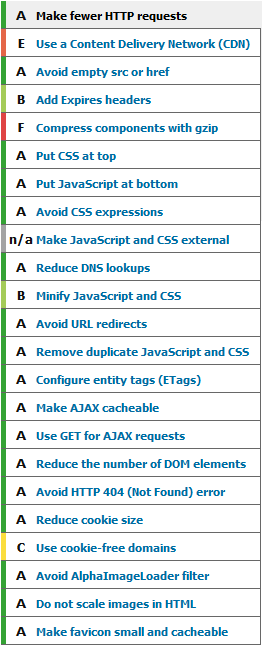
\includegraphics[keepaspectratio,scale=0.6]{images/nodeslow}}
	\subfigure[Yslow des Swift-Servers]{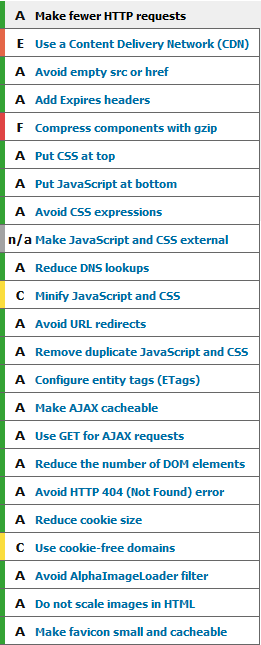
\includegraphics[keepaspectratio,scale=0.6]{images/swiftslow}}
\end{figure}

\subsection{Apache Bench}

Im ersten Schritt wird der Server mit 500 gleichzeitig durchgeführten Requests beauftrag bis insgesamt 5000 Requests abgehandelt wurden. Zur weiteren Überprüfung wird der Test mit 10.000, 20.000, 30.000, 40.000 und 50.000 zu je 500 parallelen Requests durchgeführt. Daraus wurde folgendes Ergebnis erstellt:

\begin{figure}[H]
\centering
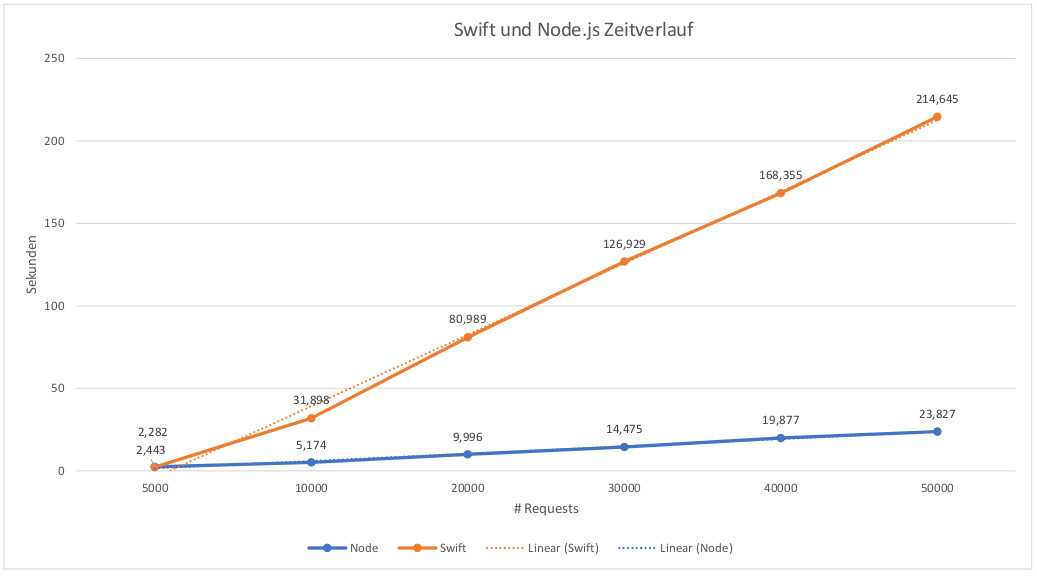
\includegraphics[keepaspectratio, scale = 0.4]{images/time.jpg}
\caption{Request-Abarbeitung von Express.js und Perfect}
\label{fig:time}
\end{figure}

\begin{table}[H]
\begin{center}
\begin{tabular}{p{8cm}p{2.5cm}p{2.5cm}}
\rowcolor{gray20}														& \textbf{Express.js}	  		& \textbf{Perfect}		\\ 
\rowcolor{gray5}		Document 											& LoginPage					& LoginPage			\\ 
\rowcolor{gray20}	Document Length										& 1.988 bytes				& 932 bytes			\\ 
\rowcolor{gray5}		Concurrency Level									& 500						& 500				\\ 
\rowcolor{gray20}	Time taken for tests [sec]								& 29,507					& 38,178			\\ 
\rowcolor{gray5}		Complete Requests									& 5.000						& 5.000				\\
\rowcolor{gray20}	Failed requests										& 0							& 0					\\ 
\rowcolor{gray5}		Total transferred [bytes]								& 11.070.000				& 6.950.000 			\\ 
\rowcolor{gray20}	HTML transferred	[bytes]								& 9.940.000					& 4.660.000			\\ 
\rowcolor{gray5}		Requests per second [\#/sec]							& 169,45					& 130,97			\\ 
\rowcolor{gray20}	Time per request [ms]	 (mean)							& 2.950,702					& 3.817,783			\\
\rowcolor{gray5}		Time per request [ms]	 (across concurrent requ.)			& 5,901						& 7,636				\\ 
\end{tabular}
\caption{Test: 5.000 Requests auf die "Login Page"} \label{tab:fivethousandrequests}
\end{center}
\end{table}

\begin{table}[H]
\begin{center}
\begin{tabular}{p{8cm}p{2.5cm}p{2.5cm}}
\rowcolor{gray20}														& \textbf{Express.js}	  		& \textbf{Perfect}		\\ 
\rowcolor{gray5}		Document 											& LoginPage					& LoginPage			\\ 
\rowcolor{gray20}	Document Length										& 1.988 bytes				& 932 bytes			\\ 
\rowcolor{gray5}		Concurrency Level									& 500						& 500				\\ 
\rowcolor{gray20}	Time taken for tests [sec]								& 172,275					& 273,546			\\ 
\rowcolor{gray5}		Complete Requests									& 50.000					& 50.000			\\
\rowcolor{gray20}	Failed requests										& 0							& 0					\\ 
\rowcolor{gray5}		Total transferred [bytes]								& 110.700.000				& 695.000.000		\\ 
\rowcolor{gray20}	HTML transferred	[bytes]								& 99.400.000				& 466.000.000		\\ 
\rowcolor{gray5}		Requests per second [\#/sec]							& 290,23					& 182,78			\\ 
\rowcolor{gray20}	Time per request [ms]	 (mean)							& 1.722,747					& 2735,462			\\
\rowcolor{gray5}		Time per request [ms]	 (across concurrent requ.)			& 3,445						& 5,471				\\ 
\end{tabular}
\caption{Test: 50.000 Requests auf die "Login Page"} \label{tab:fiftythousandrequests}
\end{center}
\end{table}

Bei dem Test wurde die Login-Page angefordert. Dabei änderte sich nur die Menge der Requests die abgehandlet werden mussten. Dadurch ergab es sich, dass die Menge der übertragenen Bytes linear anstgestiegen sind, die Zeit pro Request bei mehrmaligen durchlaufen jedoch stark schwankte. Die Differenz der Dokumentenlänge ergibt sich aus der unterschiedlich starken Kompression der Server. Somit blieb für die Abb. \ref{fig:time} nur ein Wert der sich auf beiden Seiten ändert, die \textit{Dauer des Tests}.

\section{Probleme und Lösungen}
Der Swift Server wurde auf einer VM getestet, die nur über eine CPU verfügt, wie bereits in \ref{sec:leistungsvergleich} erwähnt. Nachdem die VM um drei weitere Kerne auf 4 erweitert wurde, konnte der Server die Requests nicht mehr Ordnungsgemäß ausführen. Das lag daran, dass der Server nicht für Multitasking ausgelegt wurde, und der Server beim Bearbeiten von Requests versucht, gleichzeitig das benötigte HTML für mehrere Requests zusammenzubauen. Auf einem Rechner mit mehreren Kernen muss der Apache Bench insofern abgeändert werden, dass der \textit{Concurrency Level} auf 1 gestellt ist. Damit sind die Test jedoch wieder nicht aussagekräftig, und der Server müsste in diese Richtung überarbeitet werden. Schlussfolgernd, würde der Server auch ein viertel der Zeit benötigen, verglichen mit der derzeitigen Entwicklung.
Für die Testreihe müsste auch eine dezidierte und definierte Testumgebung festgelegt werden damit am nativen OS keine unterschiedlichen Prozesse die Ausführung der VirtualBox und damit die Test behindern bzw. beinflussen.

\chapterend


  \chapter{Zusammenfassung}
\label{chap:Zusammenfassung}

\chapterstart

Als Projekt wurde ein WebServices für Studierende der FH-Joanneum entwickelt. Dieses Service wurde in zwei Sprachen, JavaScript und Swift, implementiert. Für das entwicklen des JavaScript-Servers wurde Node.js mit dem Framework Express.js verwendet. Node.js ist eine leichte und effiziente Laufzeitumgebung für JavaScript. Für den Server selbst, wurde das Framework Express.js verwendet. Das Service wurde im Zug der Lehrveranstaltung "Rich Internet Applikation" von Michael Roitinger, Stefan Moder und Christian Hofer entwickelt. Der Server musste für die Lehrveranstalltung verschiedene Kriterien einhalten, wie das dynamische Erstellen von Webite Inhalten, das verwalten von Session, MVC-Pattern und einige weitere. Diese Kriterien dienten für den später entwickelten Swift-Server als Reverenz.\\
Um den Swift-Server zu entwickeln, musste zuerste eine Linux Distribution gefunden werden, auf der Swift kompatibel war. Aufgrund mehrerer Faktoren und schlussendlich auch aufgrund dessen, dass die Swift-Community Ubuntu empfahl, wurde für die Entwicklung Ubuntu 16.04 LTS als virtuelle Maschine im Oracels "VirtualBox" aufgesetz. Nach der Installation von Swift auf der Ubuntu Distribution, wurde der Server mit dem Swift Framework Perfect erstellt. Aus den Webframeworks Perfect, Vapor, Kitura, Zewo und Swifter wurde das Perfect Framework für diese Arbeit gewählt. Nachdem Abwegen der Vorzüge der einzelnen Frameworks, kristallisierte sich das Perfect Framework, unteranderem durch die große Menge an zusätzlichen Werkzeugen, eine detaillierte und gut dokumentierte API, gründlichen FAQs, jeder Menge Beispielcode und einer Community die auf die Fragen eingeht, heraus. Die Verwendung eines Frameworks, ist notwendig, um einen Bezug für Express.js herzustellen. Unter Verwendung von Swift gegeben Bibliotheken und den Erweiterungen von Express wurde der Swift-Server entwickelt und hinsichtlich Code, inklusive der Funktionalität von Perfect und der Abarbeitung von Request mit dem JavaScript-Server verglichen. \\
Der Leistungsvergleich erfolgte ebenfalls auf der Ubuntu Distribution. Davor wurden die Server mit YSlow verglichen und auf den gleichen Stand gebracht, um sicherzustellen, das der Vergleich auch aussagekräftig ist. Der Vergleich selbst wurde mit dem Tool "Apache Bench" durchgeführt. Dabei wurden beide Server mit 5.000, 10.000, 20.000, 30.000, 40.000 und 50.000 Requests beauftragt, wobei jeweils 500 Request zeitgleich erfolgten. Die damit erreichten Benchmarks wurden ausgewertet und ein Fazit gezogen.\\
Der Vergleich hat gezeigt, dass die Server sich sehr ähnlich sind, jedoch der Node.js Server die Requests effizienter abarbeitet. Dies ist darauf zurückzuführen, dass der Swift Server bei den I/O-Operationen blockiert und derweil keine nachkommenden Requests behandelt. Außerdem waren für den Swift-Server ein Workaround für die Templatefunktionalität, die mit Handlebars erreicht wurde, notwendig. Dieses Workaround besitzt keine Callback Funktionen wie die von Handlebars, wobie dies bei Perfect anscheindend auch nicht vorgesehen ist. Auch wenn Perfect eine stärkere Kompression aufweist, dass bei der Übermittlung vorteilhafter ist als bei Express und dem Modul Compression, benötigt es einen höheren Rechenaufwand, wodurch der Server wieder langsamer wird.

 \chapterend
  %%%%%%%%%%%%%%%%%%%%%%%%%%%%%%%%%%%%%%%%%%%%%%%%%%%%%%%%%%%%%%%%%%%%%%%%%%%%%
\chapter{Fazit und Perspektive}\label{chap:conclusion}
%%%%%%%%%%%%%%%%%%%%%%%%%%%%%%%%%%%%%%%%%%%%%%%%%%%%%%%%%%%%%%%%%%%%%%%%%%%%%
\chapterstart

\section{Fazit}

Aufgrund der Werte in der Abb.: \ref{fig:time} kann der Rückschluss gezogen werden, dass jeder zusätzliche Request einen linearen Anstieg der Durchführungsdauer zur Folge hat. Diese Aussage zeigt, dass der Swift Server sowie auch der Node.js Server die Requests synchron abarbeiten, wobei Node.js die Zeit jedoch mit Callbacks effizienter nutzt. Der Node.js Server verwendet die Zeit für I/O-Operationen, auch wenn diese synchron implementiert wurden, um nachfolgende Requests weiter zu bearbeiten. Ein großes Defizit hat der Perfect Server aufgrund des Workarounds um die Funktion von Handlebars nachzustellen. Dieses Workaround blockiert bei jedem einlesen der Partials, welche als eigene Files gespeichert sind.\\
Zusätzlich nimmt der Swift Server keinen folgenden Request engegen, bevor nicht der zurzeit bearbeitete Request abgeschlossen und gesendet wurde. Swift hat einen Vorteil durch die stärkere Komprimierung die zwar mehr Zeit beim bearbeiten von Requests benötigt, jedoch eine geringere Menge an Daten übermittelt werden müssen.

\section{Perspektive}

Als weiterführende Projekte könnte folgende Ideen umgesetz werden:

\begin{compactenum}[a)]
\item Die Verschiedenen Frameworks (Vapor, Perfect, Kitura) miteinander auf Handhabung, Skalierbarkeit, Speichermanagement usw.
\item Diese Projektarbeit, bzw. den Vergleich auf kleiner Schritte herunterbrechen um die Unterschiede in der Verarbeitung von Request zwichen Node.js und Swift festzustellen.
\item Die Server auf verschiedenen OS testen, vergleichen und bewerten.
\item Mustache weiterentwickeln, damit dieses der Funktionalität von Handlebars gleicht.
\item Die Handhabung der Callbackfunktion verbessern, da diese genauso wie bei Node.js schwer lesbar sind.
\item Perfect unterstützt das gleichzeitige Abarbeiten von Requests nicht ideal, was verbessert werden könnte, da Probleme mit dem Speichermanagement auftauchen.
\item Perfect weiterentwickeln und dem von Vapor und Zewo definierten HTTP Standard angleichen. Dabei könnte auf Basis von Perfect ein neues Framework entstehen.

\chapterend

  \appendix
  %%%%%%%%%%%%%%%%%%%%%%%%%%%%%%%%%%%%%%%%%%%%%%%%%%%%%%%%%%%%%%%%%%%%%%%%%%%%%
\chapter*{Acronyms}
\label{chap:acronyms}
%%%%%%%%%%%%%%%%%%%%%%%%%%%%%%%%%%%%%%%%%%%%%%%%%%%%%%%%%%%%%%%%%%%%%%%%%%%%%
% Which one will be the longest ...?
% ABCDE --> \begin{acronym}[ABCDE]
\footnotesize
\begin{acronym}[ABCDE]
  \acro{OS}{operating system}
  \acro{IDE}{integrated development environment}
  \acro{BSD}{Berkeley Software Distribution}
  \acro{SSA}{Static Single Assignment}
  \acro{AST}{Abstract Syntax Tree}
  \acro{SIL}{Swift Intermediate Language}
  \acro{LLVM IR}{LLVM Intermediate Representation}
  \acro{SDK}{Software Development Kit}
  \acro{URL}{Uniform Resource Locator}
  \acro{JSON}{JavaScript Object Notation}
  \acro{XML}{Extensible Markup Language}
  \acro{REPL}{read-eval-print-loop}
  \acro{CPU}{central processing unit}
  \acro{REST}{Representational State Transfer}
  \acro{WWDC}{World Wide Developer Conference}
  \acro{ARC}{Automatic Reference Counting}
  \acro{I/O}{Input / Output}
\end{acronym}
\normalsize


\printbibliography
% Add bibliography to table of contents as "References", at chapter level
% Keep this _after_ bibliography, only then the link in the TOC is correct!
\addcontentsline{toc}{chapter}{References}

\end{document}


%**********************************************************************
%**********************************************************************
